\chapter{MÉTHODOLOGIE ET DONNÉES EXPÉRIMENTALES}

Ce chapitre présente la méthodologie pour produire les données nécessaires à l'apprentissage ainsi que pour l'évaluation des modèles générés.  Il présente aussi une description des données en QuadPol réelles que nous utilisons pour évaluer les modèles issus des nombreux apprentissages et finalement, il décrit les outils matériels nécessaires à la réalisation du projet.

\section{Données synthétiques}

 L’image de référence ou image étiquette (sans chatoiement) n'est pas disponible en \textbf{RADAR}, ce qui résulte en une incapacité de réaliser une évaluation précise des effets des filtrages à l'aide d'une vérité terrain "réelle".  Afin de générer les ensembles d'entraînement et de test composés de paires d'images caractéristiques et de leurs étiquettes,  nous avons simulé le chatoiement sur des images synthétiques. La simulation du chatoiement des images  \acrsar en amplitude ou en intensité est assez simple à produire.  La partie réelle et imaginaire du retour du signal \acrsar sur les images une vue suivent chacune une  distribution  normale centrée en zéro et de variance $\sigma/2$ (voir Sec. \ref{sec:speckle}).
 
\subsection{Génération de données polarimétriques} \label{sec:cholesky}

Dans le cas des données polarimétriques, nous devons tenir compte de la corrélation entre les trois polarisations du vecteur $\Vec{k_C}$ (Eq. 2.17) .
Pipia et Fàbregas \cite{PolsarSim} proposent une procédure qui permet de produire à partir de mesures réelles de matrices de covariance, des échantillons avec le chatoiement corrélé simulé. On procèede selon les étape suivantes:
\begin{enumerate}
\item Calculer la matrice triangulaire $\simplematrix{F}$ tel que 
\begin{equation}
     \matcov = \simplematrix{F}\simplematrix{F}^{H}
\end{equation}
par la méthode de factorisation de Cholesky. La matrice $\simplematrix{F}$ est en quelque sorte une «racine carrée» de $\matcov$;
\item Générer un vecteur aléatoire $\Vec{\nu}$ suivant une loi normal complexe centrée en zéro.  La partie réelle et imaginaire du vecteur est générée indépendamment à partir d'une distribution normale centrée en zéro et de variance égale 0.5;
\item Calculer le vecteur de polarisation $\Vec{k_C}$ tel que
\begin{equation}
    \Vec{k_C}=\simplematrix{F}\Vec{\nu}
\end{equation}
\item Calculer la matrice de covariance multivue simulée
 \begin{equation}
\matcov^{\prime} = \frac{1}{L_n} \sum_{i=1}^{L_n}(\Vec{k}_{iC} \cdot \Vec{k}_{iC}^{H})
 \end{equation}
\end{enumerate}

où $L_n$ est le nombre de vues.  Dans notre cas, le nombre de vues est égale à 1 afin de simuler des données une vue.

\subsection{Signatures polarimétriques tests}

Les signatures polarimétriques ($\matcoh$) ont été calculées à partir de l'image de démonstration NASA/JPL AIRSAR en Bande L et un nombre de vues égal à 4.  Les signatures on été produites en sélectionnant initialement deux mesures représentatives pour chaque classe de diffuseur sur le plan $H/\bar{\alpha}$ (Fig. \ref{fig:sanfrancisco-airsar-halpha-diagram}).

La sélection des signatures a été faite automatiquement par la procédure suivante:

\begin{enumerate}
    \item Effectuer une décomposition $H/Alpha/\bar{\alpha}$ de l'image en QuadPol AIRSAR;
    \item Effectuer une partitionnement par k-moyennes à N classes pour chacune des classes $H/\bar{\alpha}$ de diffuseur;
\end{enumerate}

Les paramètres de l'algorithme de k-moyennes ont été fixés à N=2 et le nombre d'itérations à 10. Le clustering a été appliqué sur les 9 termes uniques de la matrice $\matcoh$. Les signatures de test correspondent aux centroïdes de chacun des clusters résultants. Le Tableau \ref{tab:sanfrancisco-coherence matrices} présente l'ensemble des matrices $\matcoh$ ainsi calculées et normalisées par le \itspanns. Dans le cas de la classe des diffuseurs ponctuels purs (Z1) nous utilisons la mesure donnée par \cite{Foucher2014}. Cette matrice correspond à une matrice de rang 1 représentant la signature d'un double-bond. Elle est non-définie sur le plan $H/\bar{\alpha}$.

\begin{figure}
  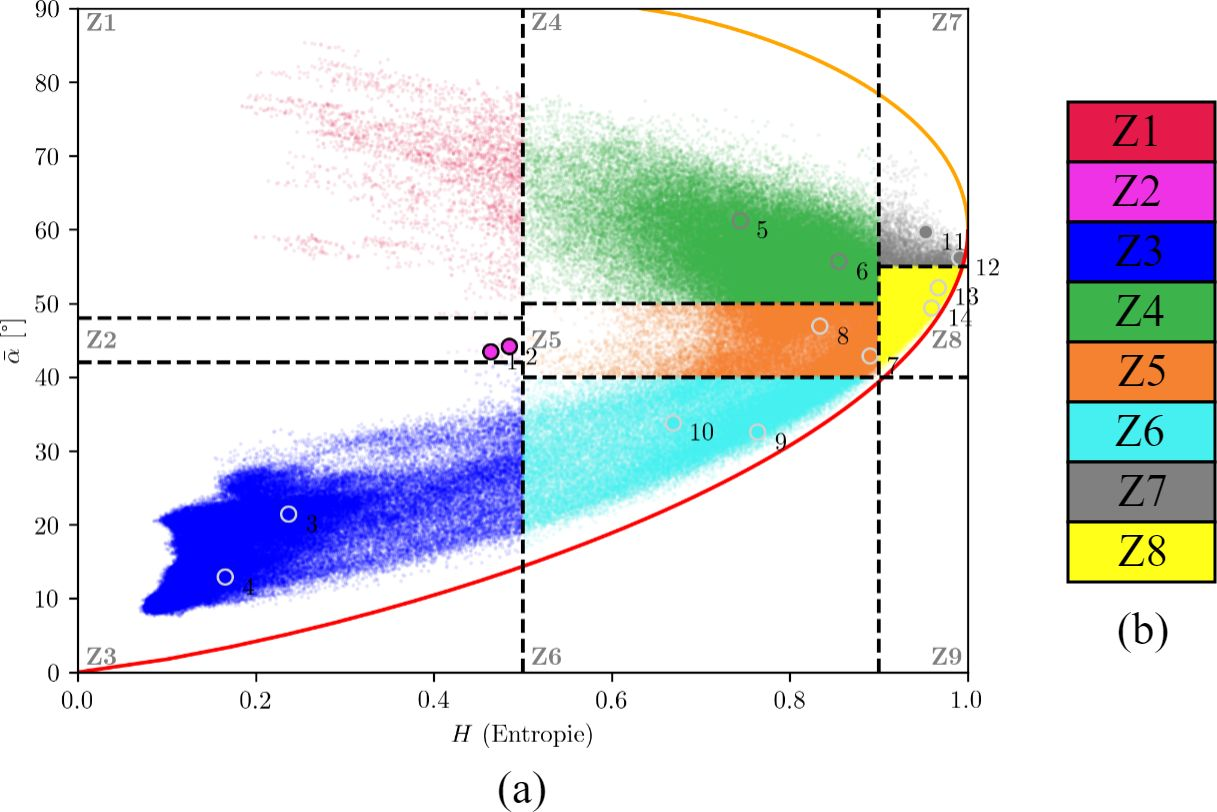
\includegraphics[width=0.90\linewidth]{figures/Chap3/halpha_sanfrancisco_diagram.jpg}
  \centering
  \caption{
  \small{
  Diagramme $H/\bar{\alpha}$ de l'image AIRSAR de la région de San Francisco. (a) Les marqueurs numérotés de 1 à 14 représente la localisation sur la plan $H/\bar{\alpha}$ de chacune des matrices de cohérence sélectionnées pour les tests (voir Tab. ~\ref{tab:sanfrancisco-coherence matrices}). (b) Légende des couleurs associées à chacune des classes de diffuseur.
  }
  }
  \label{fig:sanfrancisco-airsar-halpha-diagram}
\end{figure}

\haalphasigs

\subsection{Simulation de régions homogènes} \label{sec:simulation_de_region_homomgene}

Des images caractéristiques et des images étiquettes de taille $256\times256$ pour chaque signature polarimétrique ont été générées.  La Figure \ref{fig:shomogeneous_polarimetric_signatures} présente quelques exemples de simulation sur des régions homogènes produites à partir des matrices de cohérence calculées.  Chaque imagette présente le composé de Pauli normalisé.   Le nombre équivalent de vues (\acrenl) a été vérifié sur les trois bandes de puissance ($T_{11}, T_{22}, T_{33}$) de la matrice de cohérence \matcoh.  Ils sont consistants avec la valeur théorique pour les images une vue: $\acrenl=1$ (voir Tab. \ref{tab:homogeneous_enl_table}).

\begin{figure}
  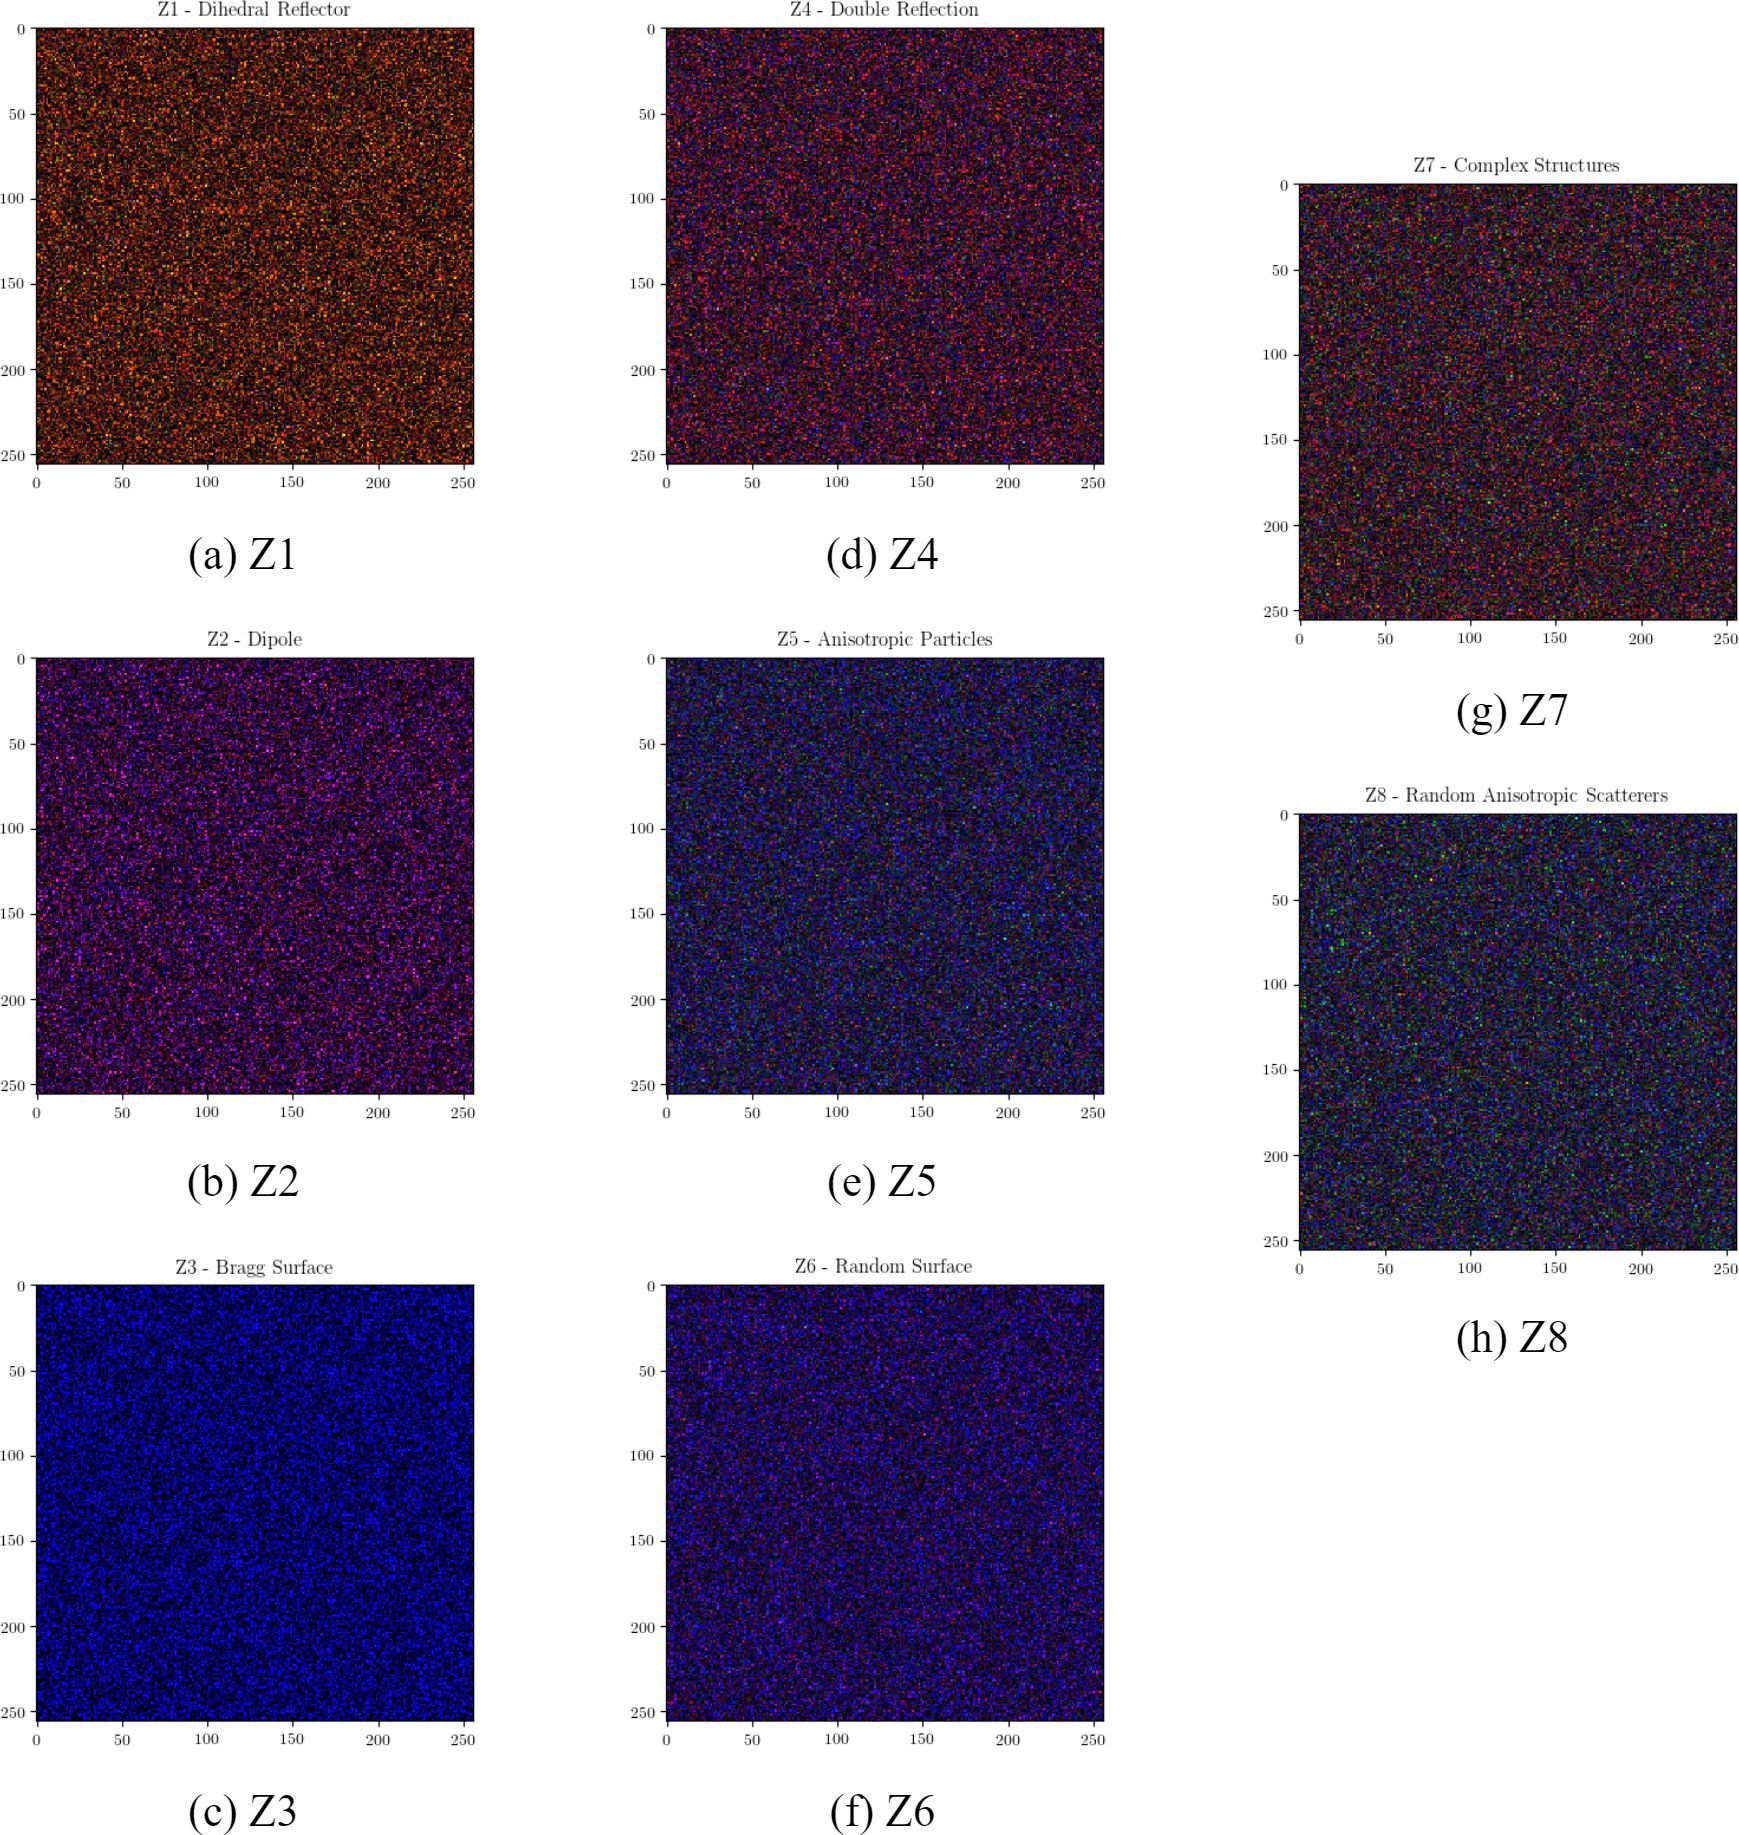
\includegraphics[width=1.1\linewidth]{figures/Chap3/homogeneous_polarimetric_signatures.jpg}
  \centering
  \caption{
  \small{Exemples des simulations de chatoiement une vue ($N=1$) de données polarimétriques sur des régions homogènes.  Le figures de (a) à (h) représentent le composé de Pauli de chacune des signatures polarimétriques sur le diagramme $H/\bar{\alpha}$. }
  }
  \label{fig:shomogeneous_polarimetric_signatures}
\end{figure}




\begin{table}[]
\begin{tabular}{|l|l|l|l|l|l|l|l|l|}
\hline
            &\textbf{Z1} & \textbf{Z2}& \textbf{Z3} &\textbf{Z4}& \textbf{Z5}& \textbf{Z6}&\textbf{Z7}&\textbf{Z8}\\ \hline\hline
$T_{11}$    & 1.006 &   0.991   &   0.994   &   1.006   &   0.999   &   0.996   &   1.007   &0.993 \\ \hline
$T_{22}$    & 1.001 &   0.995   &   0.997   &   1.006   &   1.008   &   1.001   &   0.998   &1.006  \\ \hline
$T_{33}$    & 1.001 &   0.993   &   1.005   &   1.004   &   1.002   &   1.005   &   1.000   &0.998  \\ \hline
\end{tabular}
 \caption{
  \small{Nombre de vues équivalent (\acrenl) calculé sur quelques simulations}
  }
  \label{tab:homogeneous_enl_table}
\end{table}

\subsection{Simulation de régions hétérogènes (patchwork)} \label{section:simulation_heterogeneous_regions}

\begin{figure}
  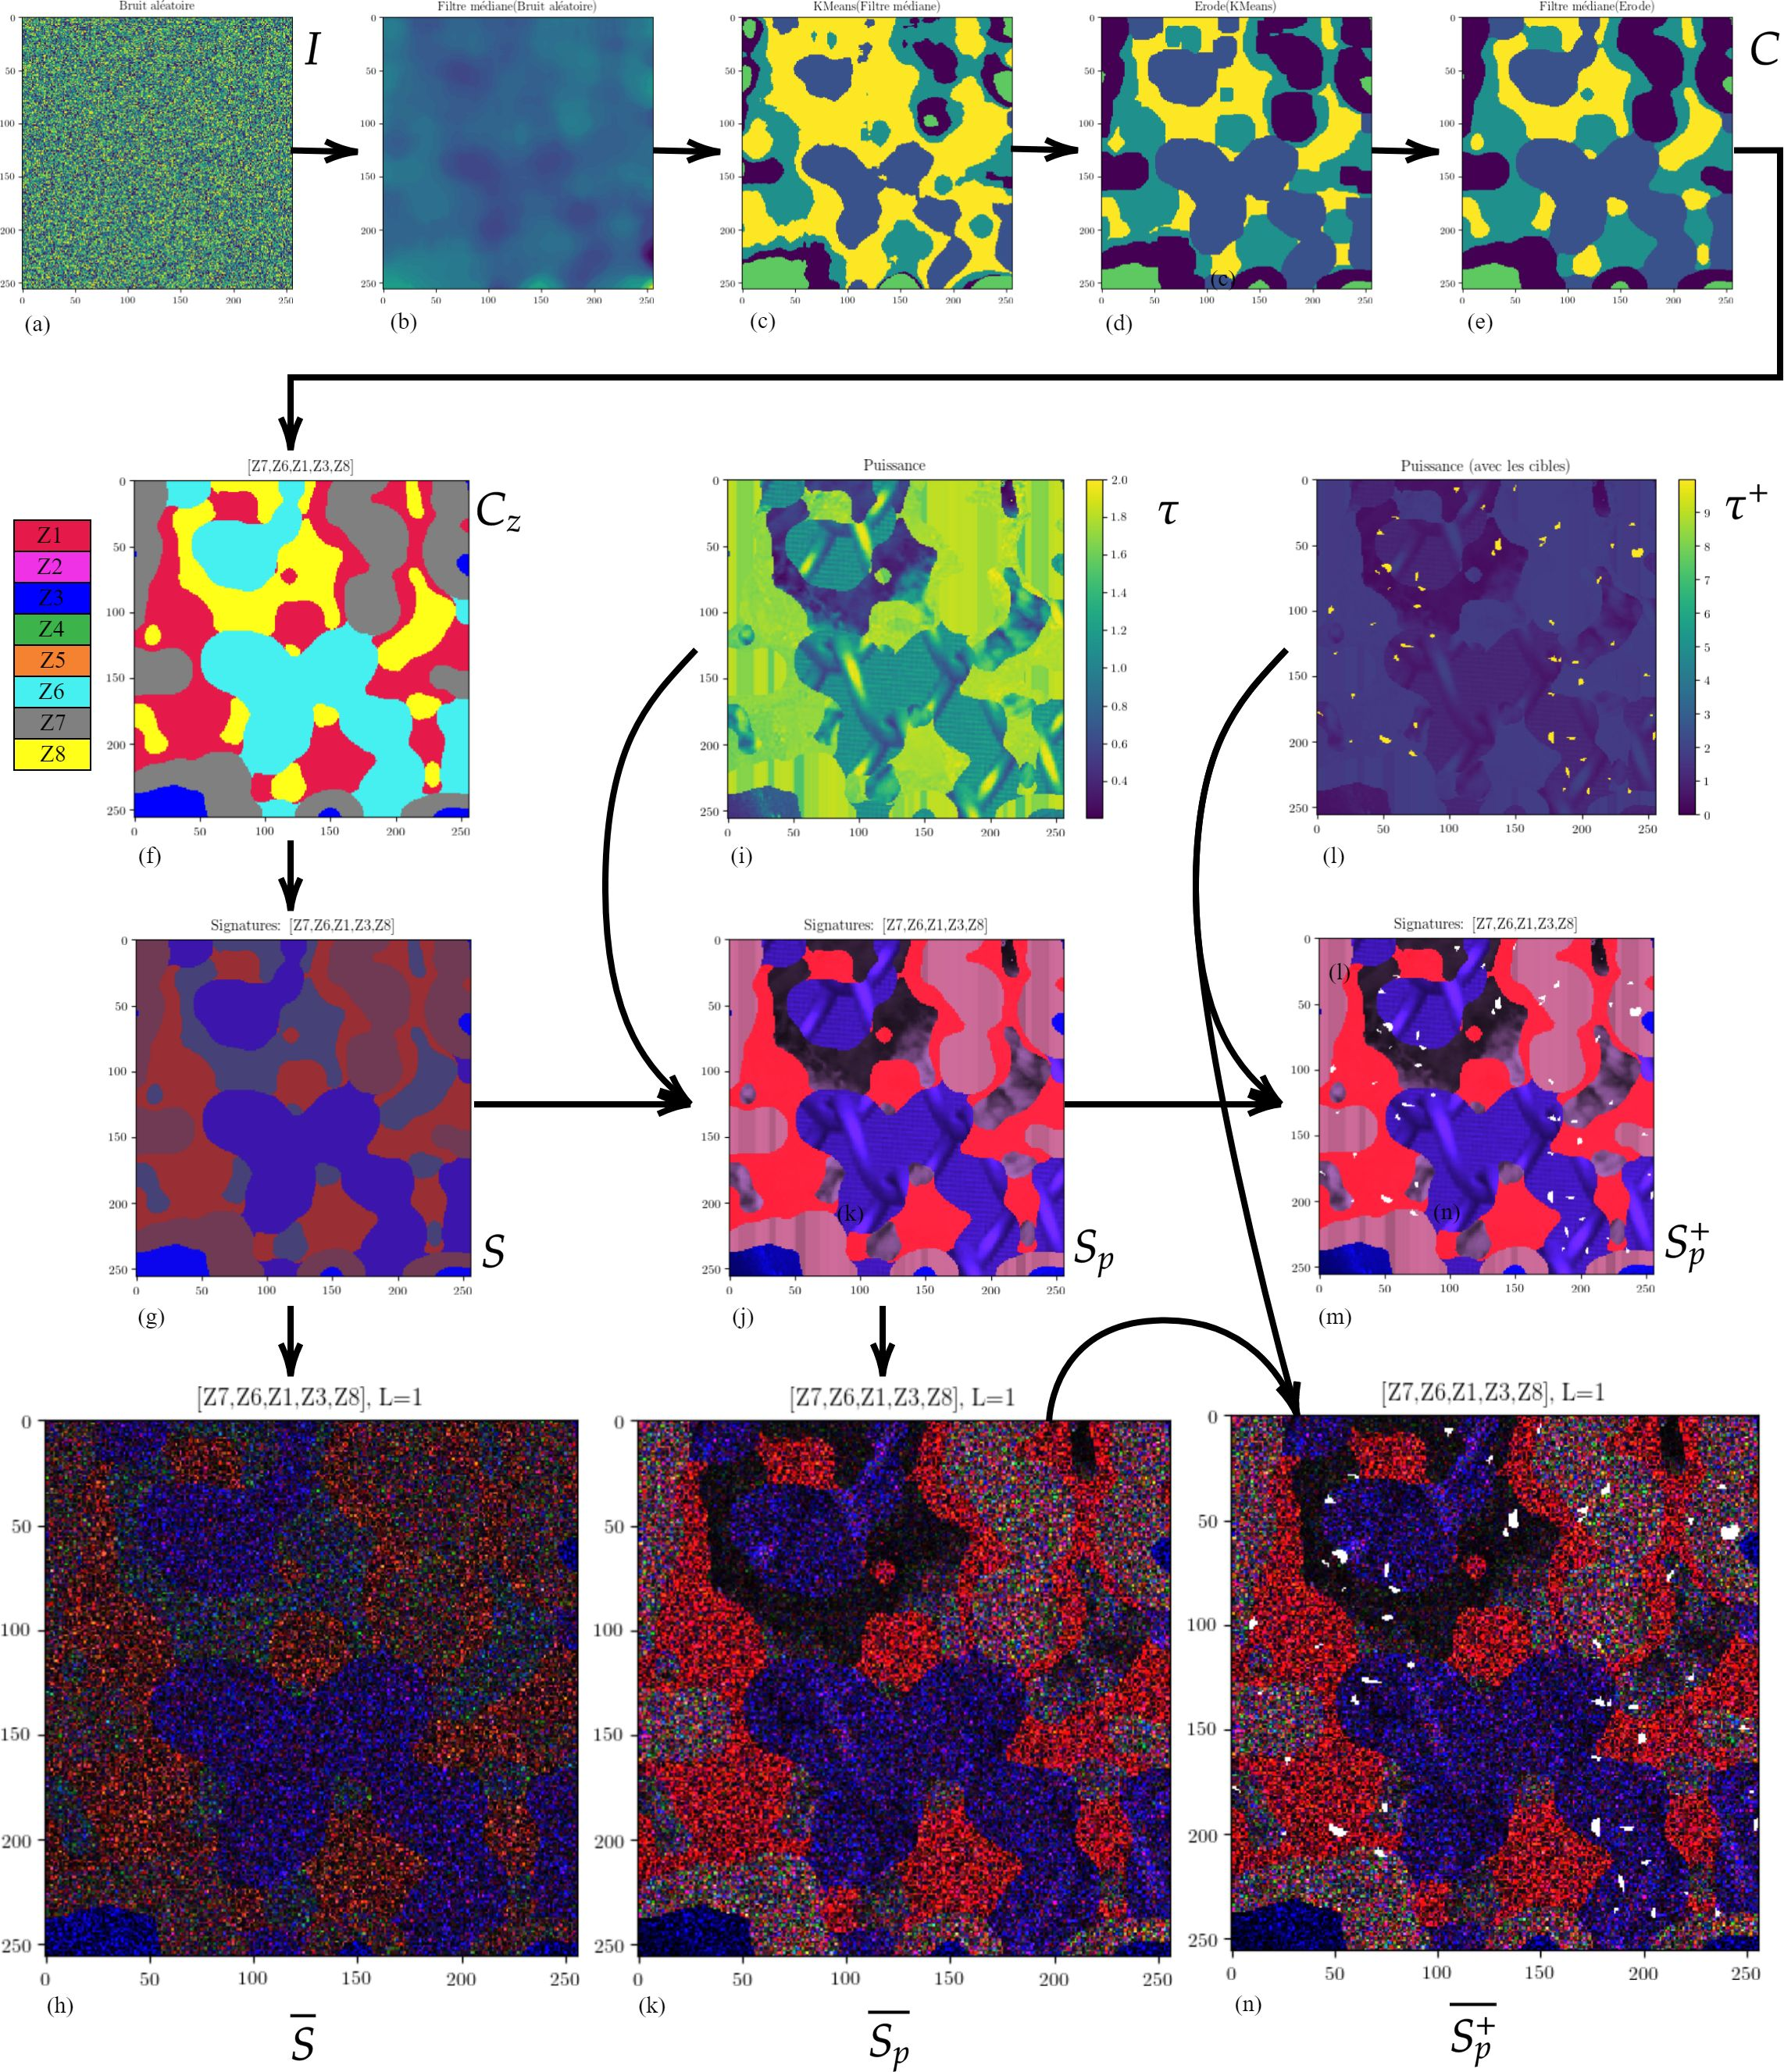
\includegraphics[width=1.1\linewidth]{figures/Chap3/samples_production_diagram.jpg}
  \centering
  \caption{
  \small{Schéma des étapes de production des simulations. }
  }
  \label{fig:samples_production_diagram}
\end{figure}

Trois types de simulation sont générés de manière aléatoire à partir des signatures polarimétriques du tableau \ref{tab:sanfrancisco-coherence matrices}, soient:
\begin{enumerate}
    \item Des simulations où la puissance demeure uniforme, ce qui génère des images avec des régions variées mais homogènes (Fig. \ref{fig:samples_production_diagram}-(h));
    \item Des simulations où la puissance est donnée par la variation de l'intensité d'images de texture,  ce qui génère des images avec des régions variées avec des intensités variables (Fig. \ref{fig:samples_production_diagram}-(k));
    \item Des simulations avec inclusions de cibles ponctuelles,  ce qui génère des images parsemées de points dont la puissance est supérieure de plusieurs ordres de magnitude que la puissance de leur voisinage (Fig. \ref{fig:samples_production_diagram}-(n));
\end{enumerate}

La méthode de création des simulations polarimétriques se divise en 3 étapes principales (Fig. \ref{fig:samples_production_diagram}).




\subsubsection{Étape 1 - Génération aléatoire d'une carte de régions homogènes}

Cette étape consiste à créer à partir d'une image de valeurs aléatoires, une carte partitionnée formée de régions homogènes.  Ces régions sont obtenues à partir d'un clustering et de transformations morphologiques appliquées à l'image. Le résultat de chacune des sous-étapes est illustré par les sous-figures (a)-(e) sur la figure principale \ref{fig:samples_production_diagram}.

\begin{enumerate}
    \item Générer une image $I$ aléatoire de taille $m \times m$ à partir d'une distribution uniforme sur l'intervalle $[0, 255]$. La dimension $m$ est fixée à $m=256$ (Fig. \ref{fig:samples_production_diagram}-(a));
    \item Filtrer $I$ par un filtre de la médiane large ($31 \times 31$).  Le filtrage aide l'étape suivante (Fig. \ref{fig:samples_production_diagram}-(b));
    \item Partitionner $I$ en régions en effectuant un apprentissage $k-moyennes$ non-supervisé à $N$ classes.  Le nombre de classes est inférieur ou égal au nombre de classes de diffuseur de la décomposition  $H/A/\bar{\alpha}$: $N \leq 8$.  L'image $C$ résultante est composée de régions appartenant à $K$ classes numérotées de 0 à $K-1$, $K$ pouvant être égal ou inférieur à $N$ (Fig. \ref{fig:samples_production_diagram}-(c));
    \item Appliquer un filtre morphologique avec l'opérateur d'érosion sur l'image $C$  pour éliminer les régions trop petites (Fig. \ref{fig:samples_production_diagram}-(d));
    \item Appliquer un second filtre de la médiane sur l'image $C$ pour adoucir les contours (Fig. \ref{fig:samples_production_diagram}-(e));
\end{enumerate}

\subsubsection{Étape 2 - Génération de l'image étiquette polarimétrique} \label{sec:gen_data}

Cette étape consiste à produire l'image étiquette $S$ de dimension $9 \times m \times m$.  Les neufs canaux correspondent aux neuf termes uniques de la matrice $\matcoh$ des signatures polarimétriques.  La forme générale de la matrice \matcoh est donnée par:

\begin{equation}
    \matcoh = 
    \begin{bmatrix}
    A   &   B+jC    &   D+jE    \\
    B-jC    &   F & G+jH    \\
    D-jE     &  G-jH  & I  
    \end{bmatrix}
\end{equation}

\vspace{5pt}

où $j$ est le nombre complexe $\sqrt{-1}$ et les coefficients $\{A, B, C, D, E, F, G, H , I\}$ sont les neuf termes uniques que nous noterons par l'ensemble $\{T_9\}$.

\begin{enumerate}
    \item Assigner aux $K$ classes de l'image $C$ une seule des huit classes de diffuseur polarimétrique $\{Z1, Z2, Z3, Z4, Z5, Z6, Z7, Z8\}$ de façon aléatoire. Cette nouvelle image $C_z$ donne pour chacun des pixels l'index de la classe polarimétrique assignée.  Elle est présentée par la sous-figure \ref{fig:samples_production_diagram}-(f).  La couleur de chacune des classes polarimétriques correspond aux couleurs de la Figure \ref{fig:sanfrancisco-airsar-halpha-diagram}. 
    \item Générér l'image $S$ des étiquettes de signatures.  Les valeurs $\{T_9\}$ de la classe polarimétrique déterminée par l'image $C_z$ sont assignées aux pixels de l'image $S$.  La sous-figure \ref{fig:samples_production_diagram}-(g) présente un exemple du composé de Pauli de l'image $S$.
\end{enumerate}

\subsubsection{Étape 3 - Génération de l'image polarimétrique une vue}

Chaque pixel de l'image $S$ des étiquettes est bruité pour former l'image polarimétrique une vue $\bar{S}$.  Dans le cas où la puissance demeure constante, la synthèse du chatoiement polarimétrique est faite pixel par pixel par l'algorithme de Pipia et Fàbregas \cite{PolsarSim} que nous avons décrit à la Section \ref{sec:cholesky}. La sous-figure \ref{fig:samples_production_diagram}-(h) présente un exemple du composé de Pauli de l'image une vue $\bar{S}$ synthétisée.

La simulation des images $S_p$ des signatures polarimétriques à puissance variable est produite en multipliant terme par terme l'image originale $S$ des signatures polarimétriques avec une image $\tau$ de texture (Fig. \ref{fig:samples_production_diagram}-(i)).  Cette image  $\tau$ est composée aléatoirement à partir de la banque de texture \textit{DTD} \cite{cimpoi14describing} (Fig. \ref{fig:dtd-example-diagram}). La nouvelle image $S_p$ des signatures polarimétriques est introduite dans le même procédé pour générer les images une vue pour synthétiser l'image une vue $\bar{S}_p$ à puissance variable  (Fig. \ref{fig:samples_production_diagram}-(j) pour $S_p$ et Fig. \ref{fig:samples_production_diagram}-(k) pour $\bar{S}_p$). 

Les images une vue $S_p^+$ et   $\bar{S}_p^+$ à puissance variable avec cibles ponctuelles sont générées en distribuant des cibles de quelques pixels de façon aléatoire sur les images. La Figure \ref{fig:samples_production_diagram}-(l) présente un exemple de distribution de cibles. La puissance des cibles demeure la même pour les deux images $S_p^+$ et $\bar{S}_p^+$,  car elle n'est pas influencée par l'effet du chatoiement.  Cette puissance est de l'ordre de 3 à 10 fois supérieur à la puissance moyenne des images. La Figure \ref{fig:samples_production_diagram}-(m) et la Figure \ref{fig:samples_production_diagram}-(n) présentent respectivement un exemple de $S_p^+$ et $\bar{S}_p^+$.  La Figure \ref{fig:polsar_simulation_examples} illustre quelques exemples de synthèses polarimétriques qui montrent la diversité des résultats issus du procédé.


\begin{figure}
  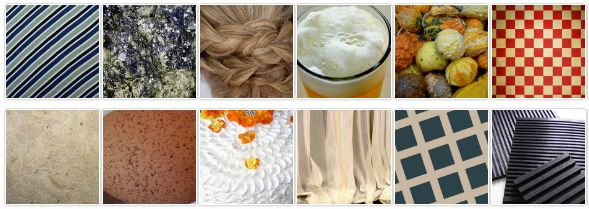
\includegraphics[width=0.85\linewidth]{figures/Chap3/texture-dataset-diagram.jpg}
  \centering
  \caption{
  \small{Exemples de texture de l'ensemble d'images \textit{Describable Textures Dataset} \cite{cimpoi14describing} utilisés pour simuler la variation de la puissance de la rétrodiffusion sur les image \acrpolsar.}
  }
  \label{fig:dtd-example-diagram}
\end{figure}

\begin{figure}
  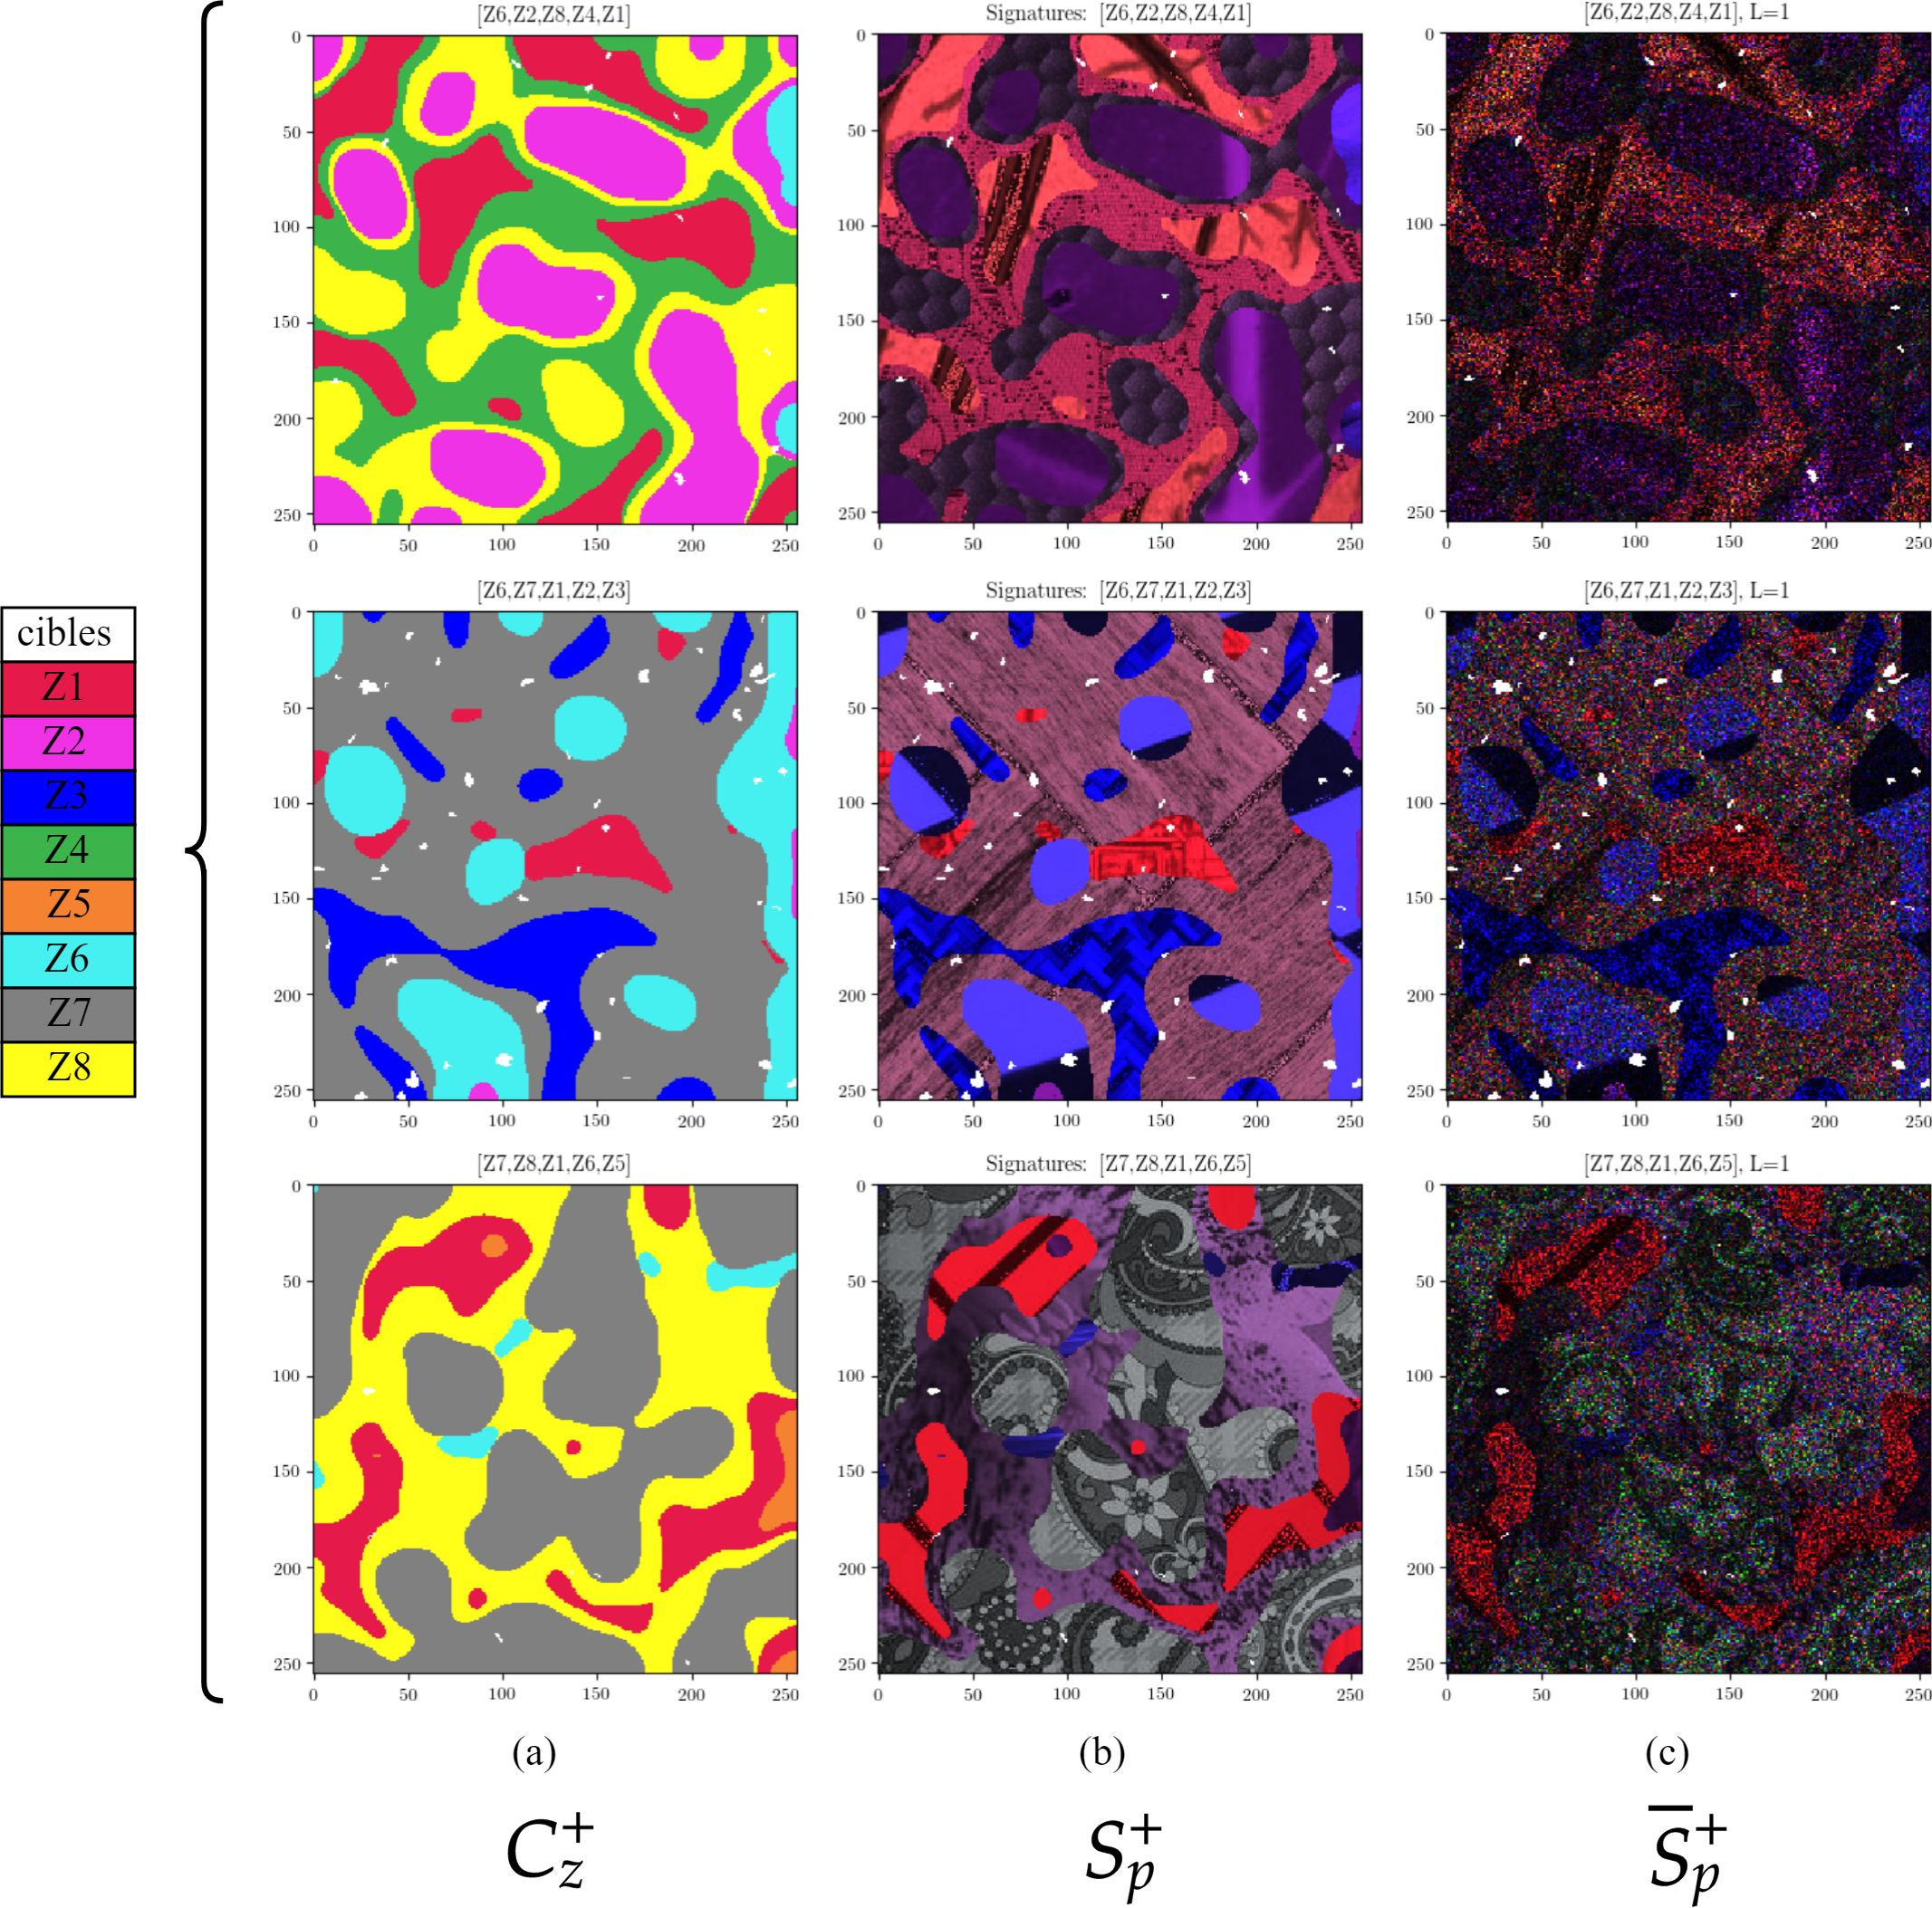
\includegraphics[width=1.0\linewidth]{figures/Chap3/polsar_simulation_examples.jpg}
  \centering
  \caption{
  \small{Trois exemples de simulation polarimétrique avec des puissances déterminées par des images de texture et avec des cibles ponctuelles incrustrées. La colonne (a) montre les étiquettes des classes de diffuseurs ($C_z^+$). La classification \halpha des régions est donnée par la légende à droite; La colonne (b) présente le composé de Pauli des images de signatures polarimétriques ($S_p^+$) sans chatoiement; La colonne (c) présente le composé de Pauli des images une vue ($\bar{S}_p^+$). }
  }
  \label{fig:polsar_simulation_examples}
\end{figure}

\section{Données réelles} \label{section:données_réelles}

Les données que nous utilisons sont des images en QuadPol acquises au-dessus de la ville de San Francisco aux États-Unis  ($37^\circ 46' 26" N, 122^\circ 25' 52" W$). La ville occupe la pointe d'une péninsule à mi-hauteur de la côte nord de la Californie, entourée sur trois côtés par des étendues d'eau: l'océan Pacifique, le détroit du Golden Gate et la baie de San Francisco. Elle est disposée dans une grille sur quelque 40 collines, pouvant atteindre des hauteurs de près de 300 mètres  (Fig. \ref{fig:sanfrancisco-roi-diagram}-a et Fig. \ref{fig:sanfrancisco-roi-diagram}-b).


Cette région est particulièrement bien étudiée dans le domaine de la recherche en \acrpolsarns.  Elle sert souvent pour l'étalonnage des nouveaux capteurs. Des images sont disponibles avec le logiciel \textit{polsapro-bio} et peuvent être téléchargées\footnote{https://www.ietr.fr/polsarpro-bio/san-francisco/} sans contraintes à des fins de recherche. Nous avons à notre disposition trois images en QuadPol  provenant de platformes satellites: RADARSAT-2, ALOS-2/PALSAR-2, GAOFEN-3. Nous avons également  l'image aéroportée AIRSAR qui définit notre région commune de recherche pour toutes les images (Fig. \ref{fig:sanfrancisco-roi-diagram}-c pour la région d'intérêt). 

\begin{figure}
  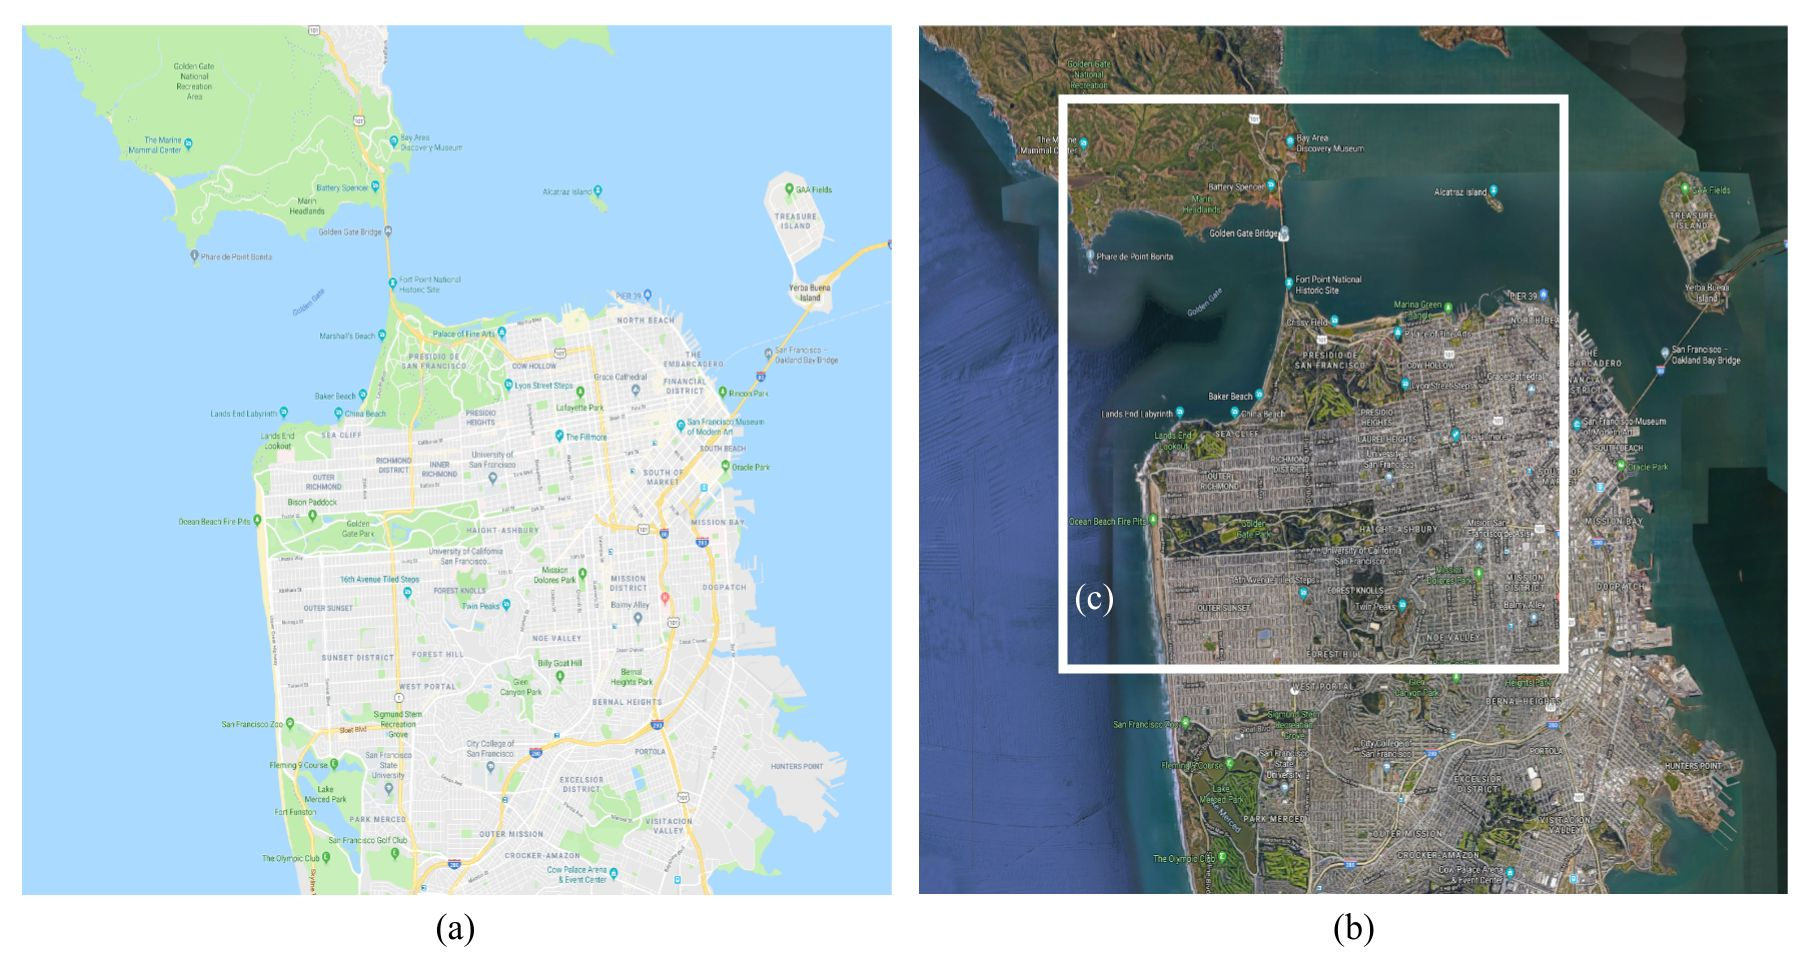
\includegraphics[width=1.0\linewidth]{figures/Chap3/sanfrancisco-roi.jpg}
  \centering
  \caption{
  \small{Région de la ville de San Francico, Californie, (ÉU). (a) Plan de la ville (source Google).  (b) Vue satellite de la région en couleur visible (source Google). (c) Le rectangle représente la région d'intérêt qui est approximativement de la taille de l'image acquise en 1999 par le capteur aéroporté AIRSAR. }
  }
  \label{fig:sanfrancisco-roi-diagram}
\end{figure}

\subsection{Image du capteur AIRSAR}

Le capteur aéroporté AIRSAR (\textit{Airborne Synthetic Aperture Radar}) était la plateforme à visée latérale \acrpolsar de recherche du Jet Propulsion Laboratory (JPL).  Son premier vol eu lieu en 1988 et sa dernière mission se termina en 2004. Il pouvait acquérir des données entièrement polarimétriques à trois longueurs d'onde radar: Bande C (5.3 GHz), Bande L (1.2 GHz) et Bande P (0.44 GHz). L'image multivue (nombre de vues = 4) acquise en 1998 est utilisée pour la synthèse des matrices \matcoh des signatures polarimétriques (Fig. \ref{fig:sanfrancisco-airsar-diagram}). 

\begin{figure}
  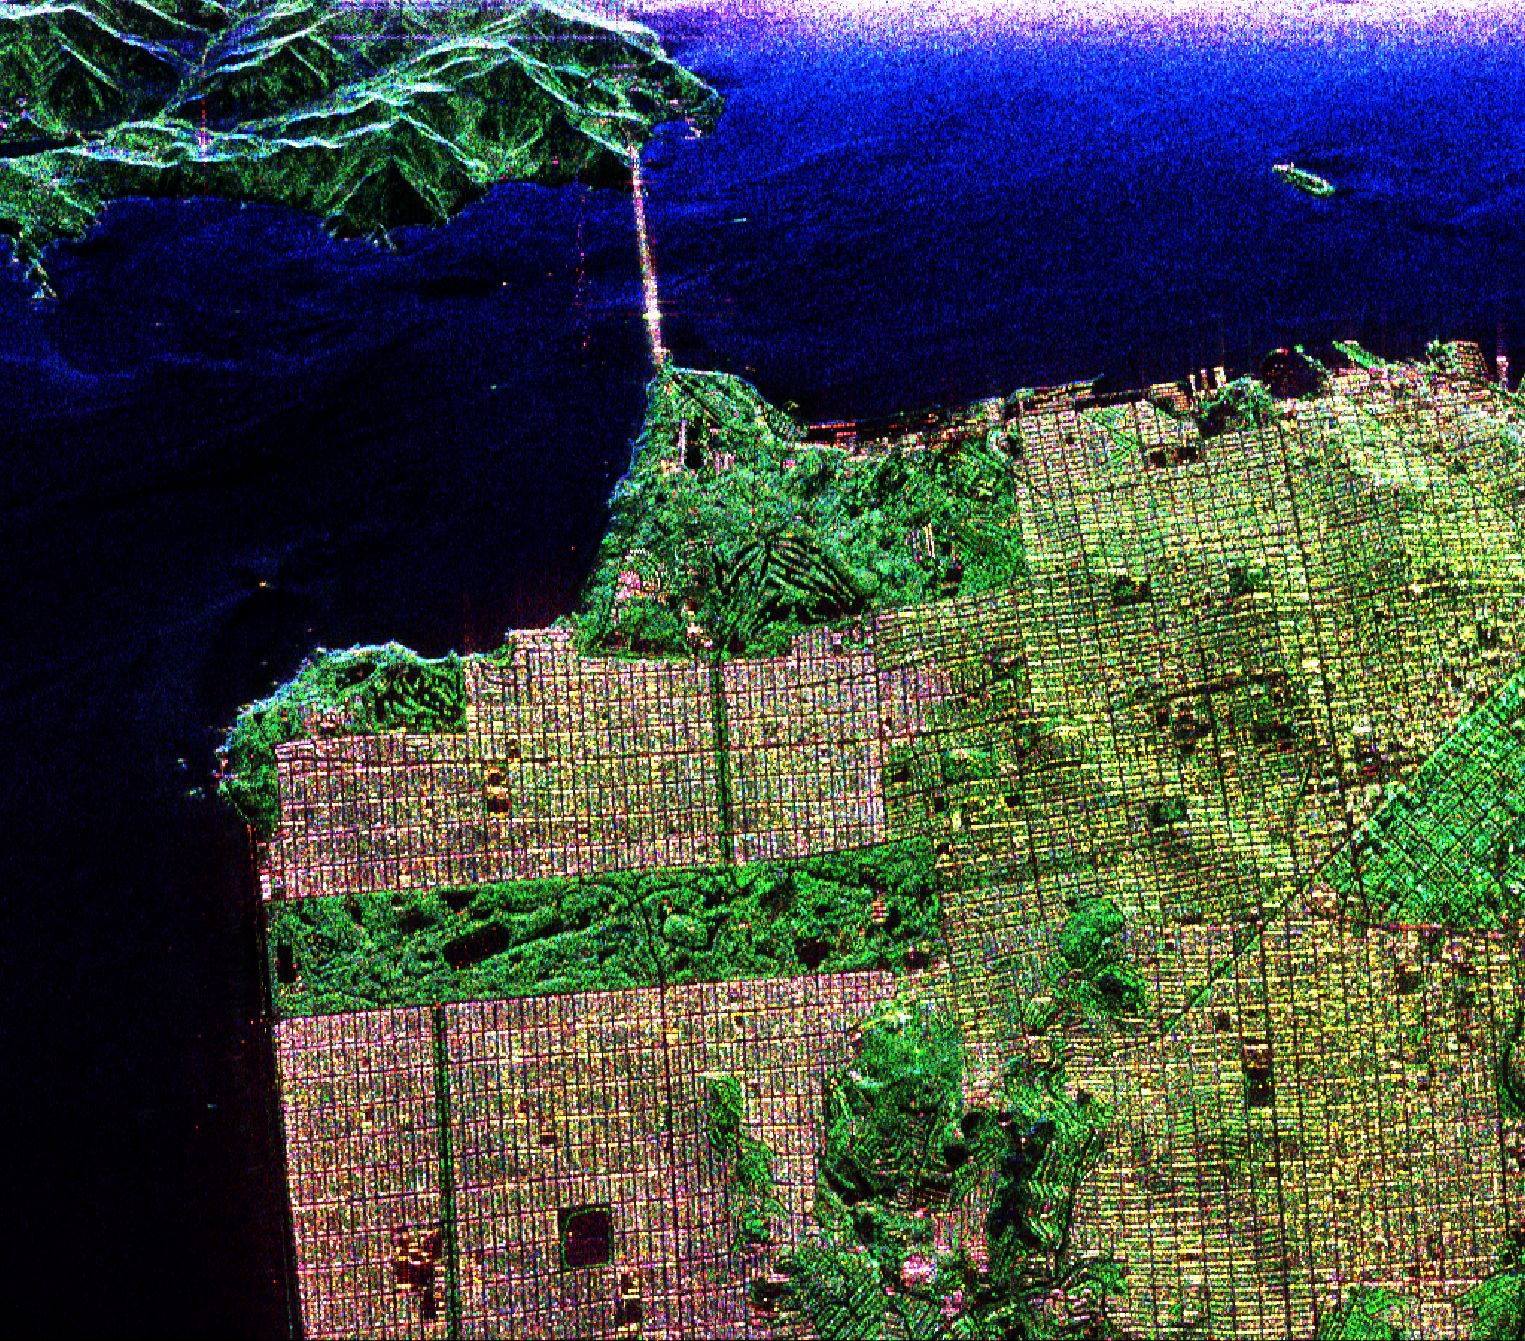
\includegraphics[width=1.0\linewidth]{figures/Chap4/AIRSAR-T3_RGB_reh.jpg}
  \centering
  \caption{
  \small{Image AIRSAR, Bande L, $\paulicomposition$}
  }
  \label{fig:sanfrancisco-airsar-diagram}
\end{figure}

\subsection{Image du capteur RADARSAT-2}

Le satellite RADARSAT-2 est un satellite canadien qui fait suite à la mission de RADARSAT-1 qui s'est terminée en avril 2013. Il a été lancé le 14 décembre 2007 et fonctionne sur la même Bande C (5.40 GHz) que son prédécesseur (5.30 GHz).  Il partage aussi les mêmes caractéristiques orbitales.  Le satellite est situé à une altitude 798 km et son orbite est hélio-synchrone avec une inclinaison de $98.16^\circ$. L'orbite a un nœud ascendant à 18 h et un nœud descendant à 6 h avec des cycles répétés de 24 jours (343 orbites). Le satellite fait 14.29 fois le tour de la terre par jour et chaque orbite a une durée de 100.75 minutes. Il donne accès aux modes de RADARSAT-1 en permettant un choix sélectif de polarisation (HH, VH, HV, VV).  A la différence de RADARSAT-1, il a des modes d’acquisition à double polarisation (HH+HV ou VV+VH) ou quadruple polarisation (HH+VH+HV+VV).  Il permet d'acquérir des images avec une résolution spatiale plus grande pouvant atteindre jusqu’à 3 mètres par pixel.
L'image une vue que nous utilisons a été acquise le 9 avril 2008, en mode fin (FQ9, $28.9^{\circ}$) avec une résolution spatiale de près de 5 mètres.  La Figure \ref{fig:sanfrancisco-radarsat2-diagram} montre la région extraite de l'image originale.

\begin{figure}
  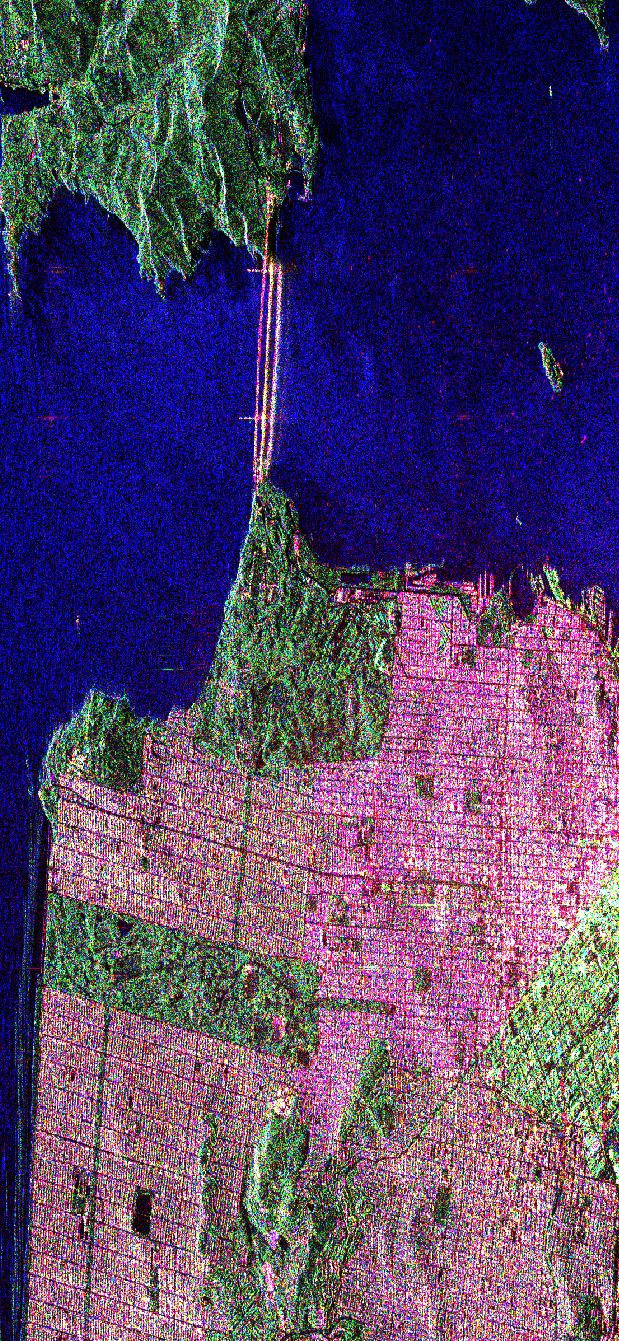
\includegraphics[height=0.95\textheight]{figures/Chap4/RADARSAT2-T3_RGB_reh.jpg}
  \centering
  \caption{
  \small{Image RADARSAT-2, Bande C, $\paulicomposition$}
  }
  \label{fig:sanfrancisco-radarsat2-diagram}
\end{figure}

\subsection{Image du capteur ALOS-2/PALSAR-2}

Le satellite ALOS-2 (Advanced Land Observing Satellite 2), également appelé Daichi-2, est un satellite japonais de 2 tonnes lancé en 2014. Il est le successeur du satellite ALOS et fonctionne sur la Bande L (1.2 GHz). Il est sur une orbite hélio-synchrone à une altitude de 628 km avec des cycles répétées de 14 jours. Il donne accès aux mêmes modes de surveillance de ALOS-1/PALSAR-1 en permettant un choix sélectif de polarisation (HH, VH, HV, VV) et des modes d’acquisition à double polarisation (HH+HV ou VV+VH) ou quadruple polarisation (HH+VH+HV+VV). Le radar PALSAR-2 constitue une mise à niveau importante du radar PALSAR, permettant des modes à plus haute résolution spatiale (1 x 3m par pixel) comparativement à 10 mètres pour son prédécesseur. L'image une vue que nous utilisons a été acquise le 6 juin 2015, avec un angle d'incidence $33.9^{\circ}$  et avec une résolution spatiale de 3 mètres.  La Figure \ref{fig:sanfrancisco-alos2-diagram} montre la région extraite de l'image originale.

\begin{figure}
  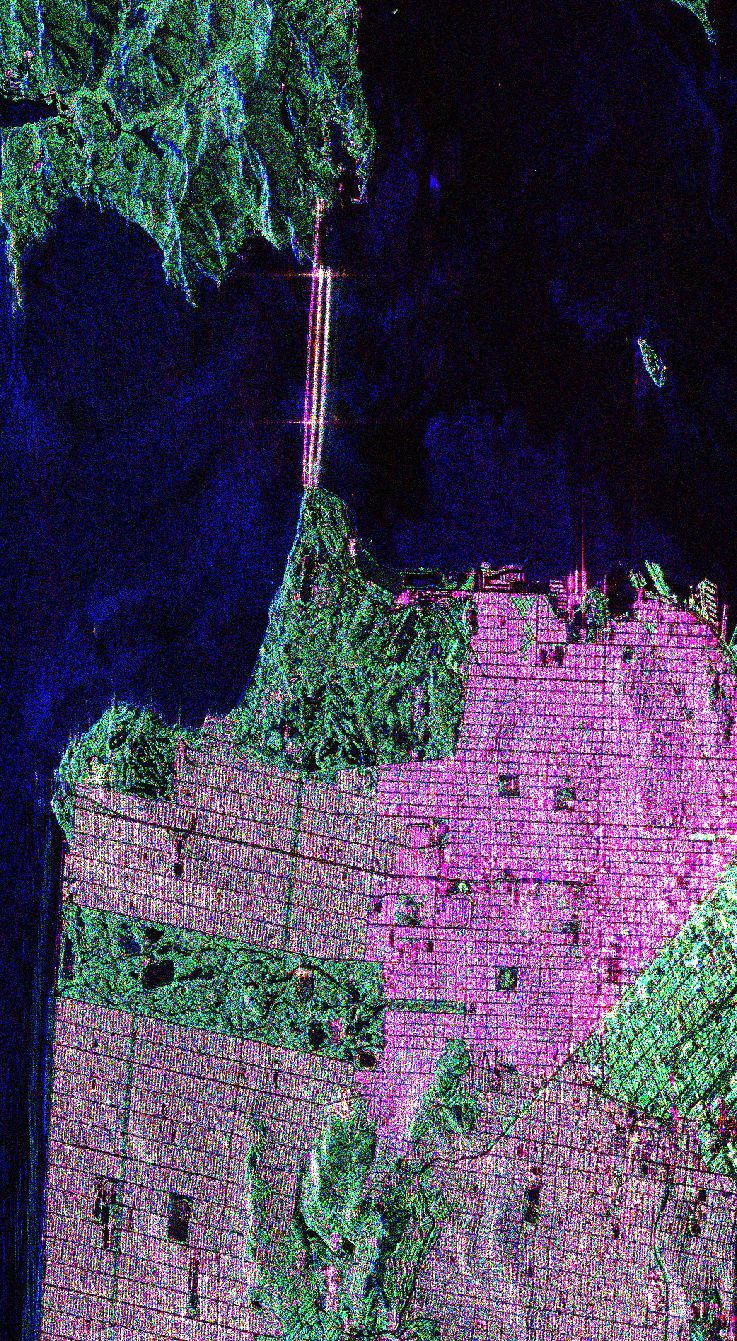
\includegraphics[height=0.95\textheight]{figures/Chap4/ALOS2-T3_RGB_reh.jpg}
  \centering
  \caption{
  \small{Image ALOS-2, Bande L, $\paulicomposition$}
  }
  \label{fig:sanfrancisco-alos2-diagram}
\end{figure}

\subsection{Image du capteur GAOFEN-3}

\begin{figure}
  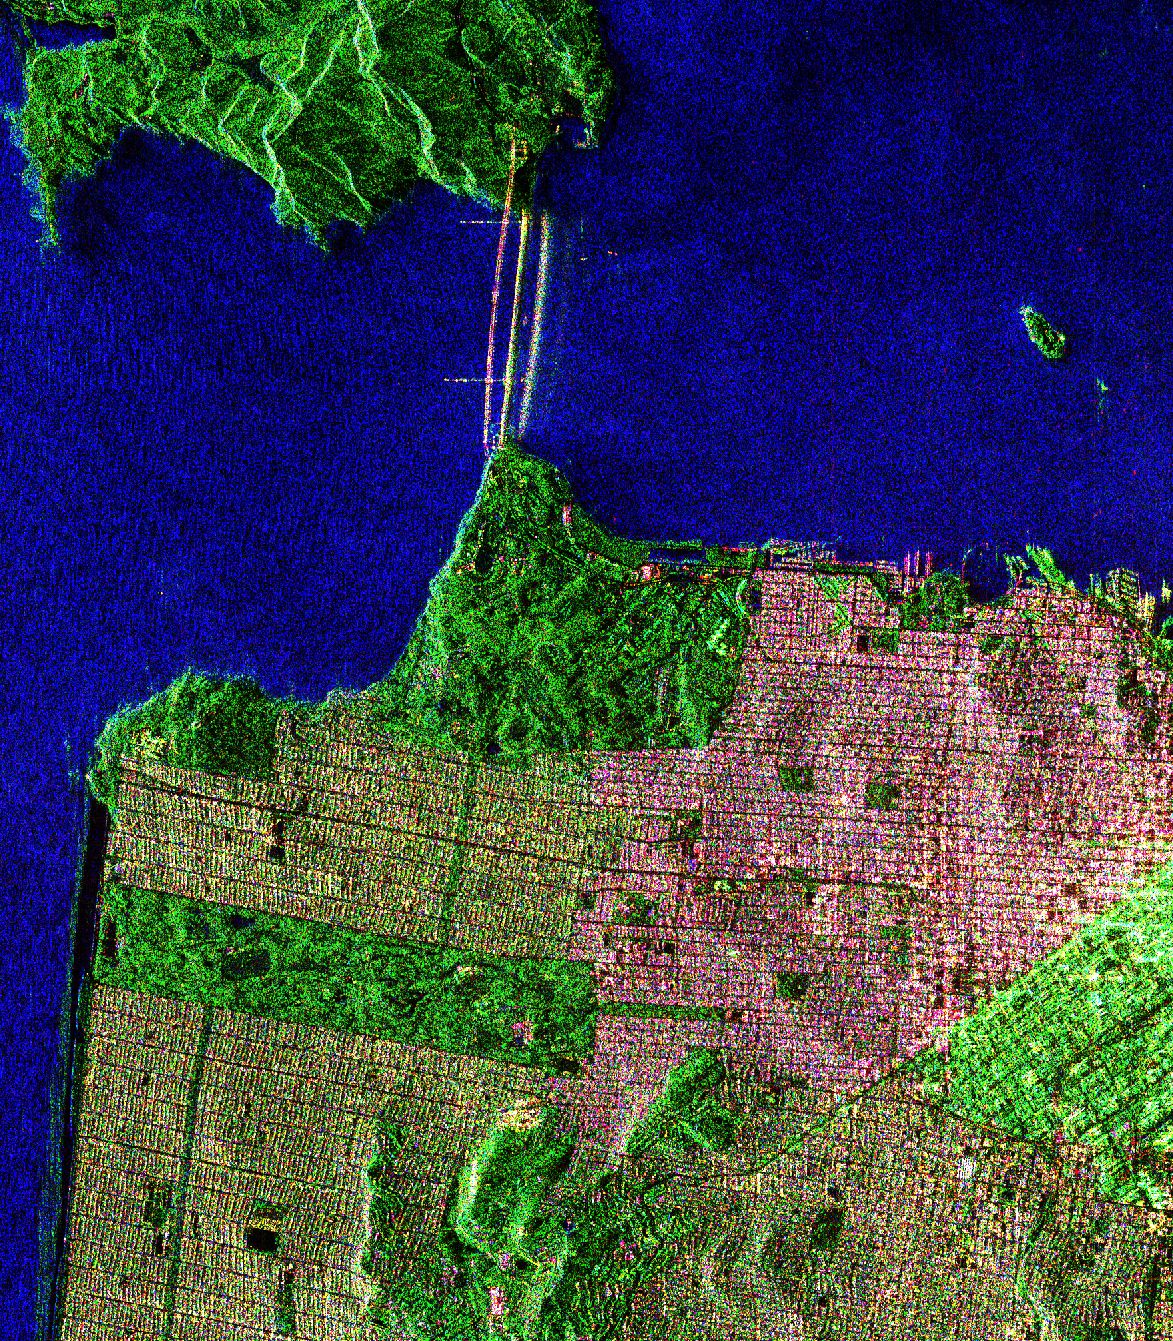
\includegraphics[width=1.0\linewidth]{figures/Chap4/GAF3-T3_RGB_reh.jpg}
  \centering
  \caption{
  \small{Image GAF-3, Bande C, $\paulicomposition$}
  }
  \label{fig:sanfrancisco-gaf3-diagram}
\end{figure}

Le satellite GAOFEN-3 (Gāofēn, haute résolution) est l'un des satellites d'observation de la terre du programme chinois High-Definition Earth Observation Satellite (HDEOS).  Ce satellite a été lancé en 2016, sur une orbite  héliosynchrone ( $98.4^\circ$) à 758 km d'altitude avec des cycles répétés de 29 jours. Il fonctionne comme RADARSAT-2 sur la Bande C (5.4 GHz) et présente des modes d'acquisition similaires.  La résolution maximale du capteur est de 1 mètre par pixel.  L'image une vue que nous utilisons a été acquise 15 septembre 2017, avec un angle d'incidence de $21.22^{\circ}$ et une résolution spatiale de près de 3 mètres.  La Figure \ref{fig:sanfrancisco-gaf3-diagram} montre la région extraite de l'image originale.

Ces trois images en QuadPol seront utilisées dans la dernière partie du mémoire pour analyser et évaluer qualitativement la performance des filtrages par \acrconvnet sur des données réelles.

\section{Apprentissage du réseau}  \label{sec:experimental_protocol}

L'objectif de l'apprentissage est d'apprendre un modèle permettant d'estimer la matrice de cohérence à partir de données polarimétriques une vue.

\subsection{Description du réseau expérimental} \label{sec:description_cnn}

Nous avons choisi d'utiliser une architecture neuronale issue du domaine de la superrésolution \cite{Yang2018DeepLF}.  Ces architectures sont facilement convertibles pour effectuer d'autres types de restauration d'image. Et parmi celles-ci, l'architecture du VDSR\cite{Kim_2016_VDSR} nous semblait tout indiquée par sa simplicité et par la démonstration qu'elle pouvait être modifiée et ajustée au filtrage des images naturelles ainsi qu'aux images \acrsarns.  L'architecture originale est inspirée des réseaux VGG \cite{vgg} qui se distinguent par l'utilisation unique de filtres de convolution $3\times3$ pour toutes les couches convolutives.  

\begin{figure}
  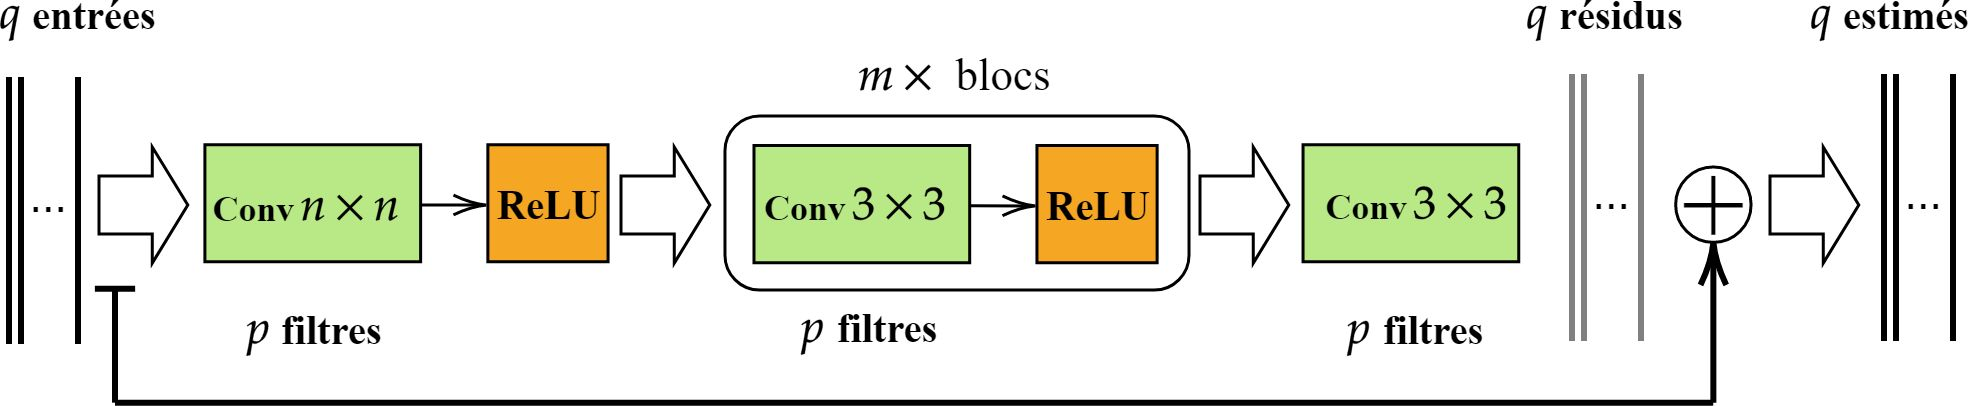
\includegraphics[width=1.0\linewidth]{figures/Chap3/cnn-experiment.jpg}
  \centering
  \caption{
  \small{Schéma de l'architecture du réseau à convolution utilisé pour les expérimentations, où $p$ est le nombre de filtres par couches, $n$ est la taille des filtres de la première couche et $m$ est le nombre de répétition du bloc pour le calcul du résidu. Le symbole $\oplus$ est l'opération de calcul du résidu.}
  }
  \label{fig:cnn-experiment-diagram}
\end{figure}

La Figure \ref{fig:cnn-experiment-diagram} présente le schéma général du réseau que nous avons adapté pour nos besoins. Il est formé de $m$ blocs convolutifs en couches cachées. Un bloc convolutif est composé  d'une couche convolutive de $p$ filtres de taille $3\times3$ suivie de la fonction d'activation \acrreluns. Un filtre opère sur une région spatiale $3\times3$ sur les $p$ cartes de caractéristiques visuelles.  La première couche est formée aussi par un bloc convolutif et opère sur les $q$ canaux de l'image d'entrée.   La dernière couche est la couche résiduelle utilisée pour la reconstruction. Elle consiste en une seule couche de $p$ filtres $3\times3$ avec $q$ sorties. La couche résiduelle est calculée grâce au saut de connections ($\oplus$) qui additionne les canaux d'entrée aux canaux de sortie.  Les cartes de caractéristiques visuelles en sortie représentent donc les images résiduelles à additionner aux images d'entrée pour les restaurer.

\subsection{Les paramètres fixes}

A la suite de certains tests préliminaires, nous gardons des paramètres constants pour l'entraînement afin que les conditions expérimentales demeurent les plus stables possibles et afin de limiter les variations (voir Tab. \ref{tab:parametres_fixes}).  Les entraînements se font sur \textbf{150} époques avec un ensemble de données de taille fixe de  \textbf{5000} échantillons pour l'apprentissage et de  \textbf{256} échantillons pour l'ensemble de validation. Une époque correspond à un cycle d'apprentissage complet sur l'intégralité de l'ensemble de données de manière à ce que chaque exemple ait été vu une fois.  La taille des échantillons est de $9 \times 64 \times 64$. Il sont créés à la volée par la méthode décrite à la Section \ref{sec:gen_data}. L'ensemble de données est par conséquent renouvelé et unique pour chaque époque.  La taille du mini-lot d'apprentissage est de  $ \textbf{9} \times 1 \times 64 \times 64$.  Nous présentons les échantillons un à la fois au réseau. Les 9 termes des matrices de cohérence sont vues comme des entrées indépendantes et dans le même ordre.  La mise à jour des paramètres est faite en calculant le gradient de l'erreur moyenné sur les 9 entrées du mini-lot. Ce qui correspond à optimiser un seul modèle pour tous termes de la matrice de cohérence. Ceci est en accord avec les principes émis par Lee et al. \cite{Lee1999} dont celui qui stipule que tous les termes de la matrice de cohérence doivent être filtrés de manière identique pour conserver la corrélation entre les différents canaux de polarisation.

Le taux d'apprentissage initial est fixé à $\lambda=10^{-3}$. Il est réduit d'un facteur de 0.1 aux époques suivantes:  40, 80, 100, 120, 130 et 140.  L'optimisation du modèle est calculé par la méthode \textit{ADAM} \cite{Kingma2014AdamAM}.  Cette méthode permet une convergence plus rapide de l'apprentissage si on la compare à la méthode classique \textit{Stochastic Gradient Descent} (SGD).

Les matrices de cohérence \matcoh utilisées pour produire les données d'entraînement sont sélectionnées à partir d'un ensemble de \textbf{6528} signatures générées aléatoirement et couvrant l'ensemble du plan $H/\bar{\alpha}$.  Les Figures \ref{fig:distribution_halpha_sigs} et \ref{fig:distribution_ha_sigs} montrent la distribution des signatures calculées. Les matrices de cohérence \matcoh utilisées pour produire les données de validation sont fournies par les signatures présentées au Tableau \ref{tab:sanfrancisco-coherence matrices}. Ces signatures ont été calculées préalablement à partir de l'image AIRSAR de San Francisco.

La fonction de coût $\epsilon$ à minimiser est l'erreur absolue entre l'estimé du modèle $\bar{y}$ et l'échantillon étiquette $y$: 
\begin{equation}
    \epsilon (y, \bar{y})= | y - \bar{y}|
\end{equation}

Cette fonction permet de faire l'apprentissage d'un modèle dont la tâche est de minimiser le biais absolu sur les 9 paramètres uniques de la matrice \matcoh.

\begin{figure}
    \centering
    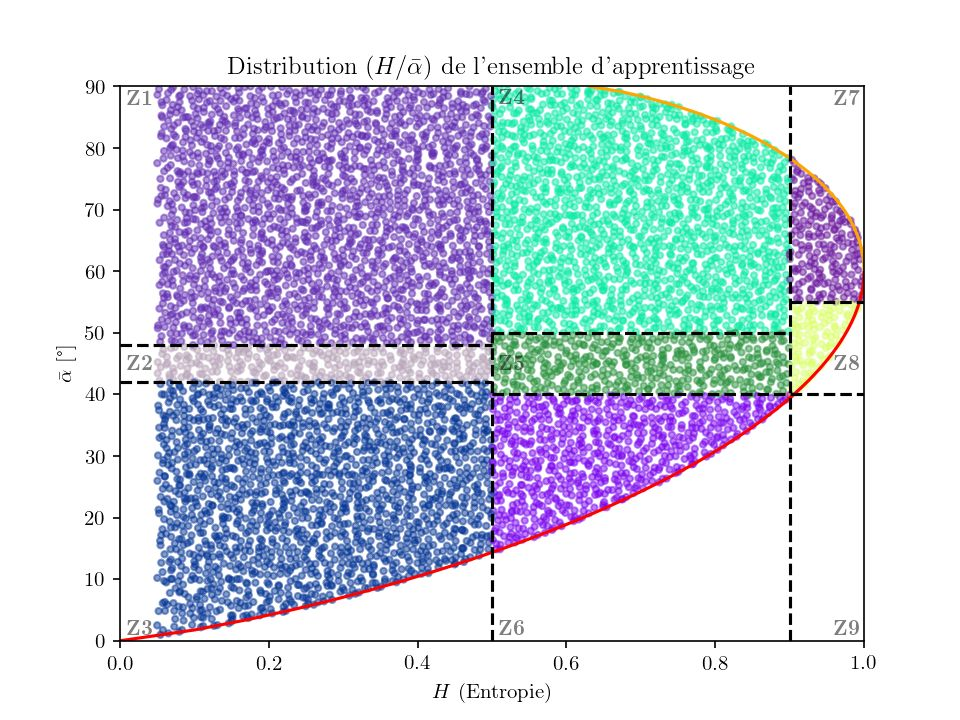
\includegraphics[width=0.85\linewidth]{figures/Chap3/train_covmatHAlpha.jpg}
    \centering
    \caption{
    \small{ 
    Distribution $H/\bar{\alpha}$ des matrices de cohérence pour la génération des données d'apprentissage.  Les couleurs représentent les différentes classes de diffuseur.}
    }
    \label{fig:distribution_halpha_sigs}
\end{figure}

\begin{figure}
    \centering
    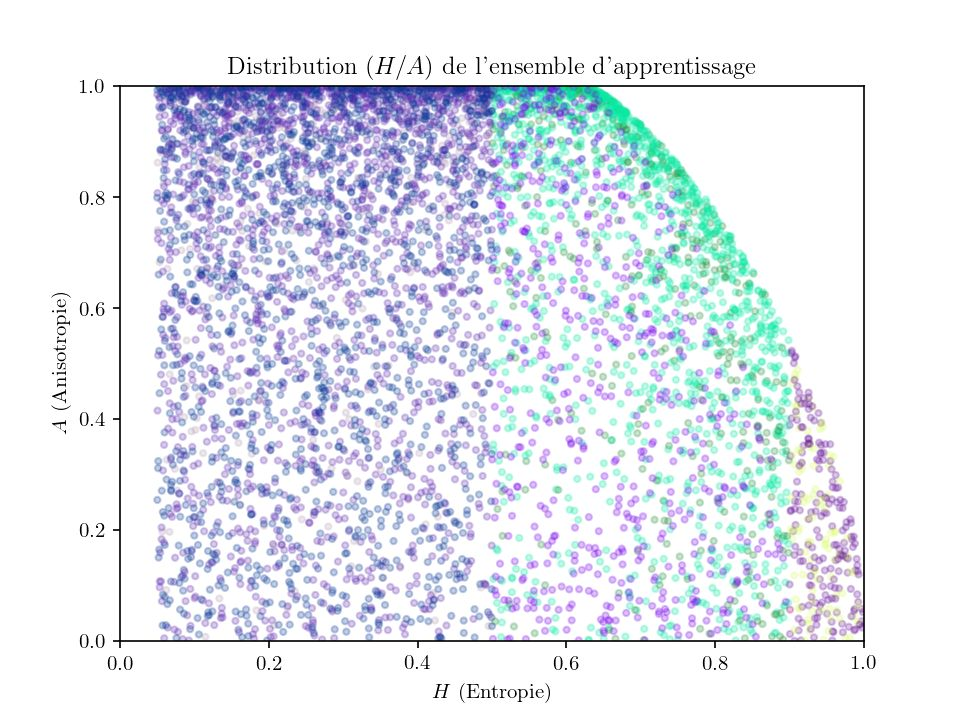
\includegraphics[width=0.85\linewidth]{figures/Chap3/train_covmatHA.jpg}
        \centering
     \caption
     {\small{ Distribution $H/A$ des matrices de cohérence pour la génération des données d'apprentissage.  Les couleurs représentent les différentes classes de diffuseur.
     }}
    \label{fig:distribution_ha_sigs}
\end{figure}


\begin{table}[]
\begin{tabular}{|l|l|}
\hline
Nombre d'époques &  150 \\ 
\hline
Taux d'apprentissage $\lambda$ &  $10^{-3}$ \\ 
\hline
Méthode de planification de réduction de $\lambda$ & Par saut de 0.1 à certaines époques précises \\  
\hline
 Méthode d'optimisation &  ADAM \\ 
  \hline
 Taille de l'ensemble d'entraînement & 5000 \\ 
 \hline
  Taille de l'ensemble de validation & 250 \\ 
 \hline
 Taille des échantillons & $9 \times 64 \times 64$ \\ 
 \hline
 Taille du mini-lot &  $ \textbf{9} \times 1 \times 64 \times 64$ (\textit{Vanilla)} \\ 
\hline
 La fonction de coût $\epsilon$ &  $L_1 = |y - \bar{y}|$  \\ 
\hline
\textit{Seeds} des générateurs aléatoires & 0 \\
\hline
\end{tabular}
\caption{\small{Paramètres qui demeurent fixes}}
\label {tab:parametres_fixes}
\end{table}

\subsection{Les paramètres testés}

Les paramètres d'apprentissage que nous faisons varier sont tous reliés à la configuration du réseau convolutif (voir Tab. \ref{tab:parametres_test}).  La taille de la convolution ($n$) de la première couche varie entre 3 et 15 à titre de comparaison avec un filtre Boxcar de même taille. Le nombre de filtres ($p$) varie de 64 à 8 pour tester le nombre minimal de paramètres par bloc convolutif.  L'impact de la hiérarchisation des caratéristiques visuelles et leur complexification est testé en faisant varier le nombre de blocs convolutifs ($m$) de 0 (aucun bloc) à 5.  Nous obtenons au total $5 \times 4 \times 5 = 120$ apprentissages distincts.

\begin{table}[]
\begin{tabular}{|l|l|}
\hline
Taille $n$ des filtres de la première couche convolutive & 3, 5, 7, 9, 11, 13, 15\\ 
\hline
Nombre $p$ de filtres par couche convolutive &  8, 16 , 32 , 64 \\ 
\hline
Nombre $m$ de blocs convolutifs  & 0, 1, 3, 5\\  
\hline
\end{tabular}
\caption{\small{Paramètres testés}}
\label {tab:parametres_test}
\end{table}

\subsection{L'estimation des paramètres polarimétriques}

La qualité des modèles comme estimateur de la matrice \matcoh est évaluée en calculant les biais sur l'estimation $\bar{\Theta}_p$ de certains paramètres polarimétriques $\Theta_p$. L'erreur $\epsilon$ de l'estimation $\bar{\Theta}_p$ sur un échantillon  $\bar{y}$ de la sortie du modèle est donnée par:
\begin{equation}
    \epsilon(\bar{y}) = \bar{\Theta}_p(\bar{y}) - \Theta_p (y)
\end{equation}

où $\Theta(y)_p$ est la valeur réelle du paramètre polarimétrique calculée à partir de la valeur étiquette ($y$) de la matrice \matcoh. Le biais sur le paramètre $\bar{\Theta}_p$ est défini par:

\begin{equation}
    \beta (\bar{\Theta}_p) = E\big[\bar{\Theta}_p(\bar{y})\big] - \Theta_p (y)
    \label{eq:bias}
\end{equation}

où $ E\big[\bar{\Theta}_p(\bar{y})\big]$ est l'espérance de l'estimation sur un échantillon. Le biais absolu relatif est donné par

\begin{equation}
     \beta_r (\bar{\Theta}_p) =\Bigg| \frac{E\big[\bar{\Theta}_p(\bar{y})\big] - \Theta(y)_p|}{\Theta_p(y)}\Bigg|
\end{equation}

où $\Theta(y)_p \neq 0$.  Dans le cas où $\beta = 0$, l'estimateur $\bar{\Theta}_p$ est dit non-biaisé. L'erreur quadratique moyenne absolue ($\textbf{EQM}$) de $\bar{\Theta}_p$ est définie par le calcul de l'espérance $E[ \cdot ]$ de la différence au carré entre l'estimation et la valeur estimée:

\begin{equation}
    \textbf{EQM} = E\big[(\bar{\Theta}_p - \Theta_p)^2\big]
    \label{eq:eqm}
\end{equation}

\vspace{5pt}

de manière similaire, l'erreur quadratique moyenne absolue relative ($\textbf{EQM}_r$) est définie comme suit:

\begin{equation}
    \textbf{EQM}_r = E\Bigg[\Bigg(\frac{\bar{\Theta}_p - \Theta_p}{ \Theta_p}\Bigg)^2\Bigg]
\end{equation}

\vspace{5pt}

Ces erreurs mesurent la divergence moyenne d'un ensemble d'estimations par rapport à la valeur réelle du paramètre. Nous pouvons aussi construire les mesures de l'erreur absolue moyenne ($\textbf{EAM}_a $) et de l'erreur absolue relative moyenne  ($\textbf{EAM}_r $) en calculant la moyenne des biais comme suit:

\begin{equation}
    \textbf{EAM}_a = E\big[|\bar{\Theta}_p - \Theta_p|\big]
\end{equation}
et
\begin{equation}
    \textbf{EAM}_r =   E\Bigg[\Big|\frac{\bar{\Theta}_p - \Theta_p}{ \Theta_p}\Big|\Bigg]
\end{equation}

\vspace{5pt}

La variance de l'estimateur $\bar{\Theta}_p$ est donnée par:

\begin{equation}
    \textbf{VAR}(\bar{\Theta}_p) = E\big[(\bar{\Theta}_p - E[\bar{{\Theta}}_p~])^2 \big]
    \label{eq:var}
\end{equation}

\vspace{5pt}

Elle mesure la divergence d'un ensemble d'estimation par rapport à la valeur moyenne de l'estimateur. A partir des Équations (\ref{eq:bias}, \ref{eq:eqm} et \ref{eq:var}), nous pouvons établir la relation suivante:

\begin{equation}
    \textbf{EQM}(\bar{\Theta}_p) = \textbf{VAR}(\bar{\Theta}_p) + ( \beta (\bar{\Theta}_p))^2
\end{equation}

\vspace{5pt}

Elle montre que l’absence de biais ($\beta=0$), à elle toute seule, ne garantit pas que l'estimateur soit bon. En effet, un estimateur sans biais mais à variance élevée peut fournir des estimations très éloignées de la
vraie valeur du paramètre, i.e. que l'erreur quadratique entre  la valeur de l'estimation et de la valeur estimée pourrait être grande. Dans le cas où nous avons plusieurs estimateurs non-biaisés, la sélection de l'estimateur le plus efficace se fait en fonction de la plus petite valeur de variance.

Une propriété importante d'un bon estimateur est sa cohérence. Elle implique que si la taille $N$ de l'échantillon grandit alors le biais tendra vers 0 et la variance aussi.  La valeur de l'estimation converge asymptotiquement vers la valeur estimée.

\subsection{L'évaluation des filtrages}

Les paramètres polarimétriques suivants sont testés par l'évaluation des biais telle que présentée à la section précédente.

\begin{enumerate}
    \item Les 9 valeurs uniques de la matrices de cohérence \matcoh;
    \item Les valeurs de la décomposition $H/A/\bar{\alpha}$;
\end{enumerate}

La valeur du nombre de vues équivalent ($\acrenl$) est évaluée à partir des termes diagonaux de la matrice \matcoh estimée sur des zones homogènes.  

La reconstruction des détails est évaluée par des mesures de distorsion entre l'image estimée et ceux de l'image étiquette. 

La conservation des cibles ponctuelles est évaluée en mesurant le changement de la forme des cibles par rapport à la vérité terrain.

\subsection{La comparaison des filtrages}

Les résultats des estimations de la matrice \matcoh des modèles produits sont comparés principalement avec deux filtres polarimétriques:

\subsubsection{Le filtre Boxcar}

Le filtre multilook \textbf{Boxcar} pose comme hypothèse que le signal est homogène autour d'un pixel donné.  Il fait la moyenne des $n$ pixels appartenant à son voisinage défini par une fenêtre rectangulaire. C'est le filtre de chatoiement le plus simple et le plus rapide. Il correspond aussi à l’estimation du maximum de vraisemblance de la matrice de covariance et ce sans biais ni distorsion. Par contre, l'hypothèse du signal stationnaire n'est pas valable pour tous les pixels, en particulier dans les cas des cibles ponctuelles et des contours.  Dans ces cas le Boxcar peut donner de mauvais résultats en raison du mélange de pixels hétérogènes. Le filtre se comporte comme un filtre passe-bas. Il réduit la résolution spatiale et génère une image floue. Cet effet indésirable est particulièrement perceptible pour les cibles ponctuelles fortes en énergie car elles apparaissent étendues proportionnellement à la taille de la fenêtre de filtrage.

\subsubsection{Le filtre adaptatif de Lee affiné}

 Le filtre Lee affiné (\textbf{Refined Lee}) est un filtre d’erreur minimale moyenne (MMSE) développé sur la base du modèle de bruit multiplicatif \cite{Lee1999}. Un inconvénient majeur du filtre MMSE est que le bruit de chatoiement près des arêtes fortes n’est pas filtré de manière adéquate. Pour compenser ce problème, le filtre de Lee affiné utilise une fenêtre non carrée pour faire correspondre la direction des arêtes. Le filtre utilise une fenêtre glissantes $7 \times 7$ (ou $9 \times 9$, $11 \times 11$). L'une des huit fenêtres alignées sur les arêtes est sélectionnée pour filtrer le pixel central. Seuls les pixels de la zone non contenue dans la fenêtre alignée sur les contours sont utilisés dans le calcul du filtrage. Le filtre se déroule sur trois étapes de traitement:

\begin{enumerate}
    \item \textbf{Sélection de la fenêtre alignée sur les arêtes}:
    Pour chaque pixel, l'image du \itspan est utilisée pour sélectionner la fenêtre alignée sur les arêtes;
    \item \textbf{Calcul du poids du filtrage}: Un filtre évaluant les statistiques local sur l'image de \itspan est appliqué pour calculer le poids du filtrage $b$;
    \item \textbf{Filtrage de la matrice de covariance}:  Le même poids $b$ et la même fenêtre sélectionnée sont utilisés pour filtrer indépendamment et également chacun des éléments de la matrice $Z$.  La matrice filtrée est donnée par:
    \begin{equation}
        \hat{Z} = \bar{Z} + b (Z-\bar{Z})   
    \end{equation}
    où  $\bar{Z}$ est la moyenne locale de la matrice calculée à partir des pixels sous la fenêtre alignée.

\end{enumerate}
Nous comparons aussi avec d'autres filtres disponibles dans le sofware ESA-SNAP utilisé pour faire le traitement d'images en QuadPol.

\section{Le matériel} \label{sec:hardware_software}

Tout au long du projet nous avons utilisé plusieurs logiciels, nous donnons une courte description de chacun.

\begin{enumerate}
    \item \textbf{PYTHON \footnote{https://www.python.org}}
    
     Python est un langage de programmation \textit{open source} créé par Guido van Rossum en 1991. Il s’agit d’un langage interprété, qui ne nécessite donc pas d’être compilé pour fonctionner. Un programme   interpréteur permet d’exécuter le code Python sur n’importe quel ordinateur. Il permet de facilement importer de nouvelles bibliothèques logicielles de traitement et d'analyse.  L'ensemble de nos traitements sont réalisées sous forme de scripts python. La version de python que nous utilisons est la version 3.6;
     
     \item \textbf{PYTORCH \footnote{https://pytorch.org}}
     
     PyTorch est une bibliothèque logicielle Python \textit{open source} d'apprentissage machine qui s'appuie sur Torch (en) développée par Facebook. PyTorch permet d'effectuer les calculs tensoriels nécessaires pour l'apprentissage profond. Les calculs sont optimisés et effectués soit par le processeur (CPU) soit, lorsque c'est possible, par un processeur graphique (\acrgpuns) supportant CUDA. 
     Cette bibliothèque est au coeur du développement de nos scripts d'entraînement. La version de PyTorch que nous utilisons est la version 1.1;

    \item \textbf{ESA SNAP Toolbox \footnote{https://step.esa.int/main/toolboxes/snap}}
    
    SNAP est un logiciel \textit{open source} en JAVA fourni par l'Agence Spatial Européenne (ESA) pour l'exploitation des données d'observation de la Terre. Le logiciel est pourvue d'une boîte à outils spécialisée pour la manipulation des images \acrpolsarns. La boîte à outils Sentinel-1 (S1TBX) comprend un ensemble d’outils de traitement, des lecteurs et des rédacteurs de produits de données, ainsi qu’une application d’affichage et d’analyse permettant de gérer l’archive des données des missions \acrsar de l’ESA, notamment SENTINEL-1, ERS-1 et 2 et ENVISAT, ainsi que des données \acrsar tierces d’ALOS PALSAR, TerraSAR-X, COSMO-SkyMed et RADARSAT-2. Les différents outils de traitement peuvent être exécutés indépendamment à ligne de commande et où à partir de l'interface graphique. La boîte à outils comprend aussi des outils pour l’étalonnage, le filtrage du chatoiement, la coregistration, l’orthorectification, le mosaïquage, la conversion de données, l'analyse polarimétrique et l’interférométrique des données.  La version de SNAP que nous utilisons est la version 6.0.4;
    
    \item \textbf{SNAPPY Python Toolbox}
    
    SNAPPY est une bibliothèque logicielle python qui donne accès à l'API JAVA de SNAP.  Elle permet à même un script python l'utilisation des opérateurs de traitement des boites à outils de SNAP. La version de SNAPPY que nous utilisons est la version 6.0.4;
    
\end{enumerate}

L'apprentissage profond demande en général un matériel spécialisé pour être calculé efficacement.  En particulier l'ordinateur doit être muni d'une carte graphique avec un \acrgpu compatible pour l'utilisation de PyTorch.  Dans le cadre de ce projet nous avons utilisé deux systèmes pour les traitements:

\begin{enumerate}
    \item \textbf{Un système de prototypage}:
    
    Ordinateur de bureau;
    
    Carte graphique: GeForce GTX 1080 (8GB);
    
    Mémoire: 32G;
    
    CPU: 8 $\times$ Intel(R) Core(TM) i7-7700K CPU @ 4.20GHz;
    
       Il a servi à la conception et au débuggage des scripts python;

    \item \textbf{Un système de production}:
    
    Grappe de \acrgpu du CRIM\footnote{Centre de Recherche Informatique de Montréal (www.crim.ca)} (7 \acrgpu utilisés)
    
    Cartes graphiques par machine: 3 $\times$ GeForce GTX 1080-TI (11GB)
    
    Mémoire par machine: 125G
    
    CPU par machine: 18  $\times$ Intel(R) Core(TM) i9-7980XE CPU @ 2.60GHz
    
    La grappe a servi à la production en parallèle des modèles des différentes expériences;
    
\end{enumerate}

\section{Conclusion}

Nous avons présenté dans ce chapitre l'ensemble des outils mathématiques pour produire les données et évaluer les résultats.  Ainsi que le outils matériels nécessaires pour la réalisation du projet. Nous avons décrit la génération des données simulées et les données réelles que nous utilisons pour évaluer les différents modèles produits au cours des nombreuses expérimentations.